%% v2.2 [2016/03/25]
\documentclass[paper]{ieice}
\usepackage[pdftex]{graphicx,xcolor}% for pdflatex
%\usepackage[dvipdfmx]{graphicx,xcolor}% for platex or uplatex
\usepackage[fleqn]{amsmath}
\usepackage{newtxtext}
\usepackage[varg]{newtxmath}
\usepackage{cite}

\setlength\textfloatsep{5pt}

%% <local definitions>
\def\ClassFile{\texttt{ieice.cls}}
\newcommand{\PS}{{\scshape Post\-Script}}
\newcommand{\AmSLaTeX}{%
 $\mathcal A$\lower.4ex\hbox{$\!\mathcal M\!$}$\mathcal S$-\LaTeX}
\def\BibTeX{{\rmfamily B\kern-.05em
 \textsc{i\kern-.025em b}\kern-.08em
  T\kern-.1667em\lower.7ex\hbox{E}\kern-.125emX}}
\hyphenation{man-u-script}
\makeatletter
\def\tmpcite#1{\@ifundefined{b@#1}{\textbf{?}}{\csname b@#1\endcsname}}%
\makeatother
%% </local definitions>

\field{A}
\vol{98}
\no{1}
\SpecialSection{\LaTeXe\ Class File for the IEICE Transactions}



\setlength\textfloatsep{5pt}

\title{\LARGE \bf
A Tutorial and Review of Automobile dToF LiDAR SoCs: \\Evolution of Next-Generation LiDARs
}

\authorlist{%
 \authorentry{Kentaro YOSHIOKA}{n}{labelA}\MembershipNumber{}
}
\affiliate[labelA]{The author is with Keio University}

\begin{document}

\maketitle
\thispagestyle{empty}
\pagestyle{empty}


%%%%%%%%%%%%%%%%%%%%%%%%%%%%%%%%%%%%%%%%%%%%%%%%%%%%%%%%%%%%%%%%%%%%%%%%%%%%%%%%
\begin{summary}
% TODO: より論文を表すように変える必要あり。
LiDAR is a distance sensor that plays a key role in realizing Advanced Driver-Assistance Systems (ADAS).
In this paper, we present a tutorial and review of automotive LiDAR from the aspect of circuit systems.
We discuss the breakthrough in ADAS LiDARs through comparison with the first-generation LiDAR systems, which were conventionally high-cost and had an immature performance. We define current high-performance and low-cost LiDARs as next-generation LiDAR systems, which have significantly improved the cost and performance by integrating the photodetector, the readout circuit, and the signal processing unit into a single SoC.

This paper targets reader who is new to ADAS LiDARs and will cover the basic principles of LiDAR, also comparing with ranging methods other than dToF.
In addition, we discuss the development of this area through the latest research examples such as the 2-chip approach, 2D SPAD array, and 3D integrated LiDARs.

\end{summary}

\begin{keywords}
LiDAR, dToF, ADAS, automotive, SPAD, TDC, ADC.
\end{keywords}
%%%%%%%%%%%%%%%%%%%%%%%%%%%%%%%%%%%%%%%%%%%%%%%%%%%%%%%%%%%%%%%%%%%%%%%%%%%%%%%%
\section{Introduction}
\qquad Humans have better sensors and decision-making mechanisms than most modern hardware and software systems. Even though, we make incredibly childish mistakes from time to time; such mistakes have irreversible consequences, especially when driving a car. In Japan alone, the number of fatalities and injuries in traffic accidents in 2021 reached 2,636 and 361,768, respectively\cite{keisatsu}. Since it is impossible to reduce human errors to zero, Advanced Driver-Assistance Systems (ADAS) technologies are developed to compensate for such errors. As a milestone, SAE has set five levels for automated driving as shown in Table \ref{sae} \cite{sae}. For example, as of 2022, Level 0-1 automated driving, such as automatic braking and lane-keeping, is available in many commercial vehicles. To name a few examples, Tesla has released a Level 2 partially automated driving function, and Honda also equipped their products with Level 3 equivalent automated driving functions (although the use of such functions are still limited)\cite{honda}. Thus, driving functions are being transferred from human drivers to machine-controlled systems in a long termed view.

There are two main approaches to automated driving: 1) driving by constantly recognizing surrounding objects and situations like a human\cite{tesla}, and 2) by utilizing a prerecorded 3D map of the environment and estimating the ego position by fitting the sensed 3D data to the prerecorded map \cite{montemerlo2008junior}. While the former can drive in an environment without any mapping information, there is a risk that an unexpected misdetection, e.g. overlooking the gore points, may cause a severe consequence. On the other hand, while the latter requires recorded mapping information, it can mitigate the above accidents by labelling the possible driving region in advance. 
In particular, a high-quality depth sensor is essential for the latter automated driving system. In addition, the high-resolution distance sensor can be used to recognize surrounding cars and pedestrians through point cloud object detection \cite{lang2019pointpillars, qi2018frustum},  simultaneously obtaining distances between the objects.

\begin{table}[!t]
\centering
\caption{Six levels of automated driving set by SAE.}
 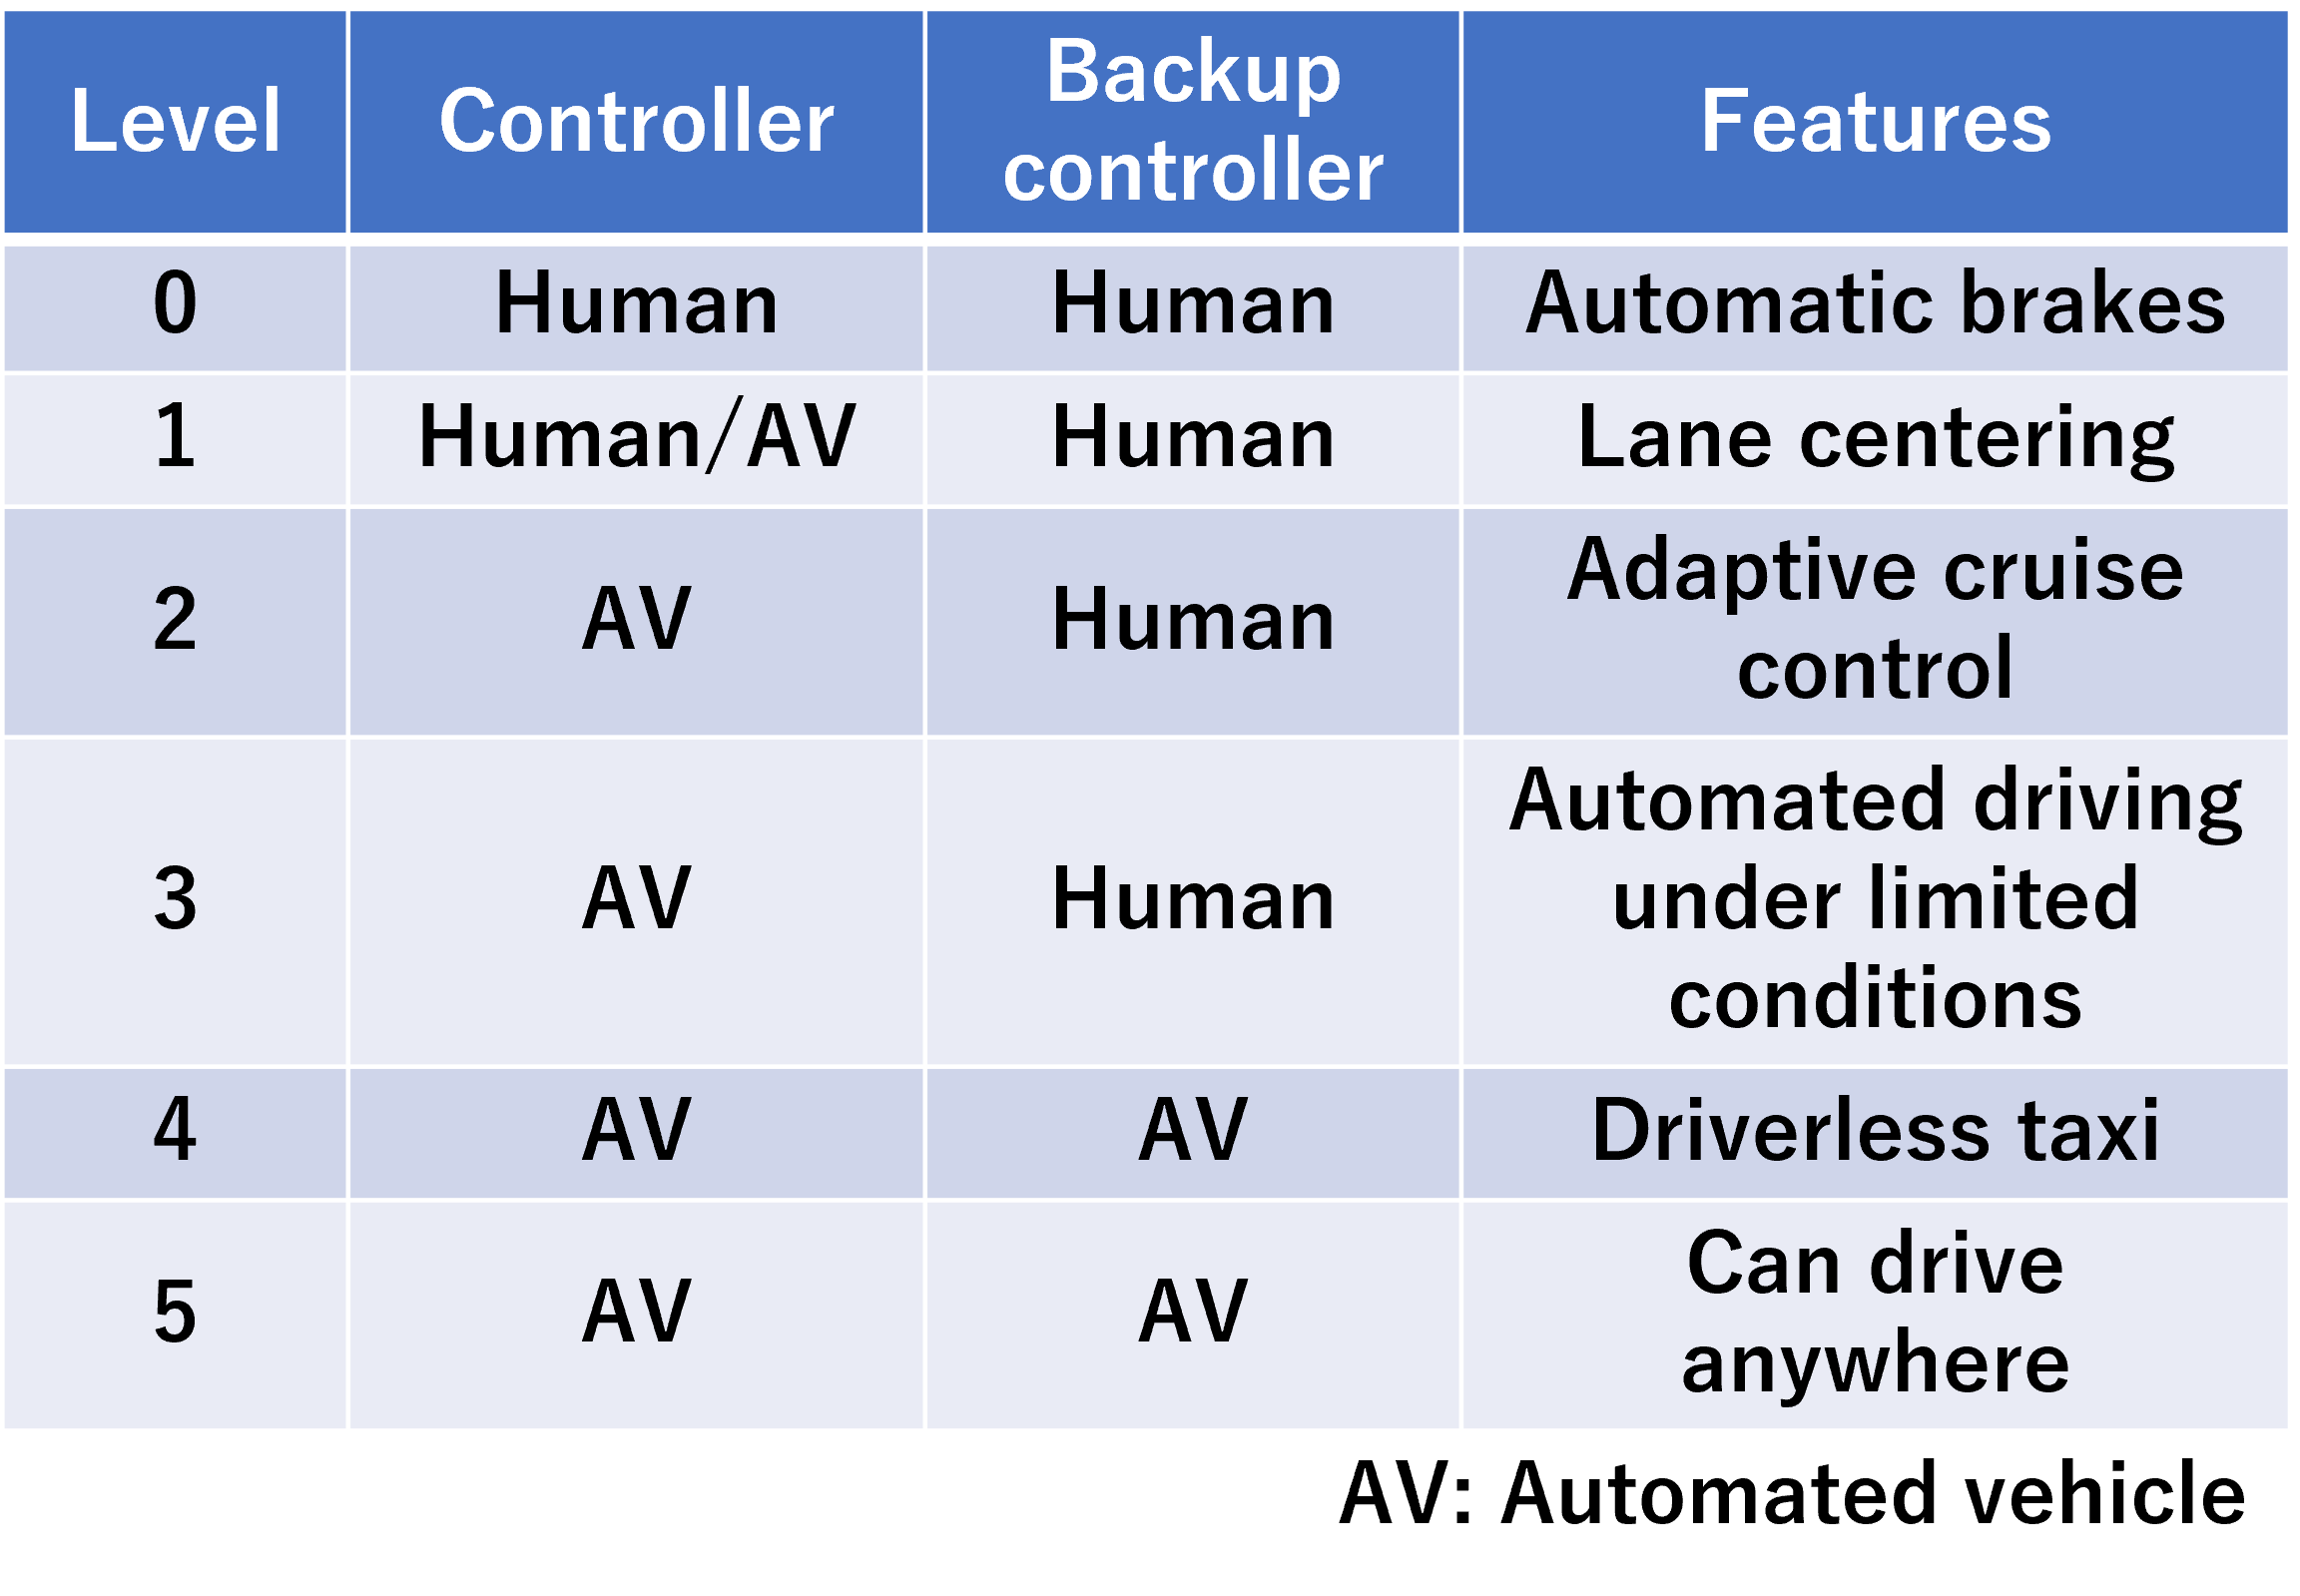
\includegraphics[width=0.5\textwidth]{figs/ses.png}
\label{sae}
\end{table}

\begin{table}[!t]
\centering
\caption{A distance sensor used in typical ADAS systems are shown. A tradeoff exist between cost and performance.}
 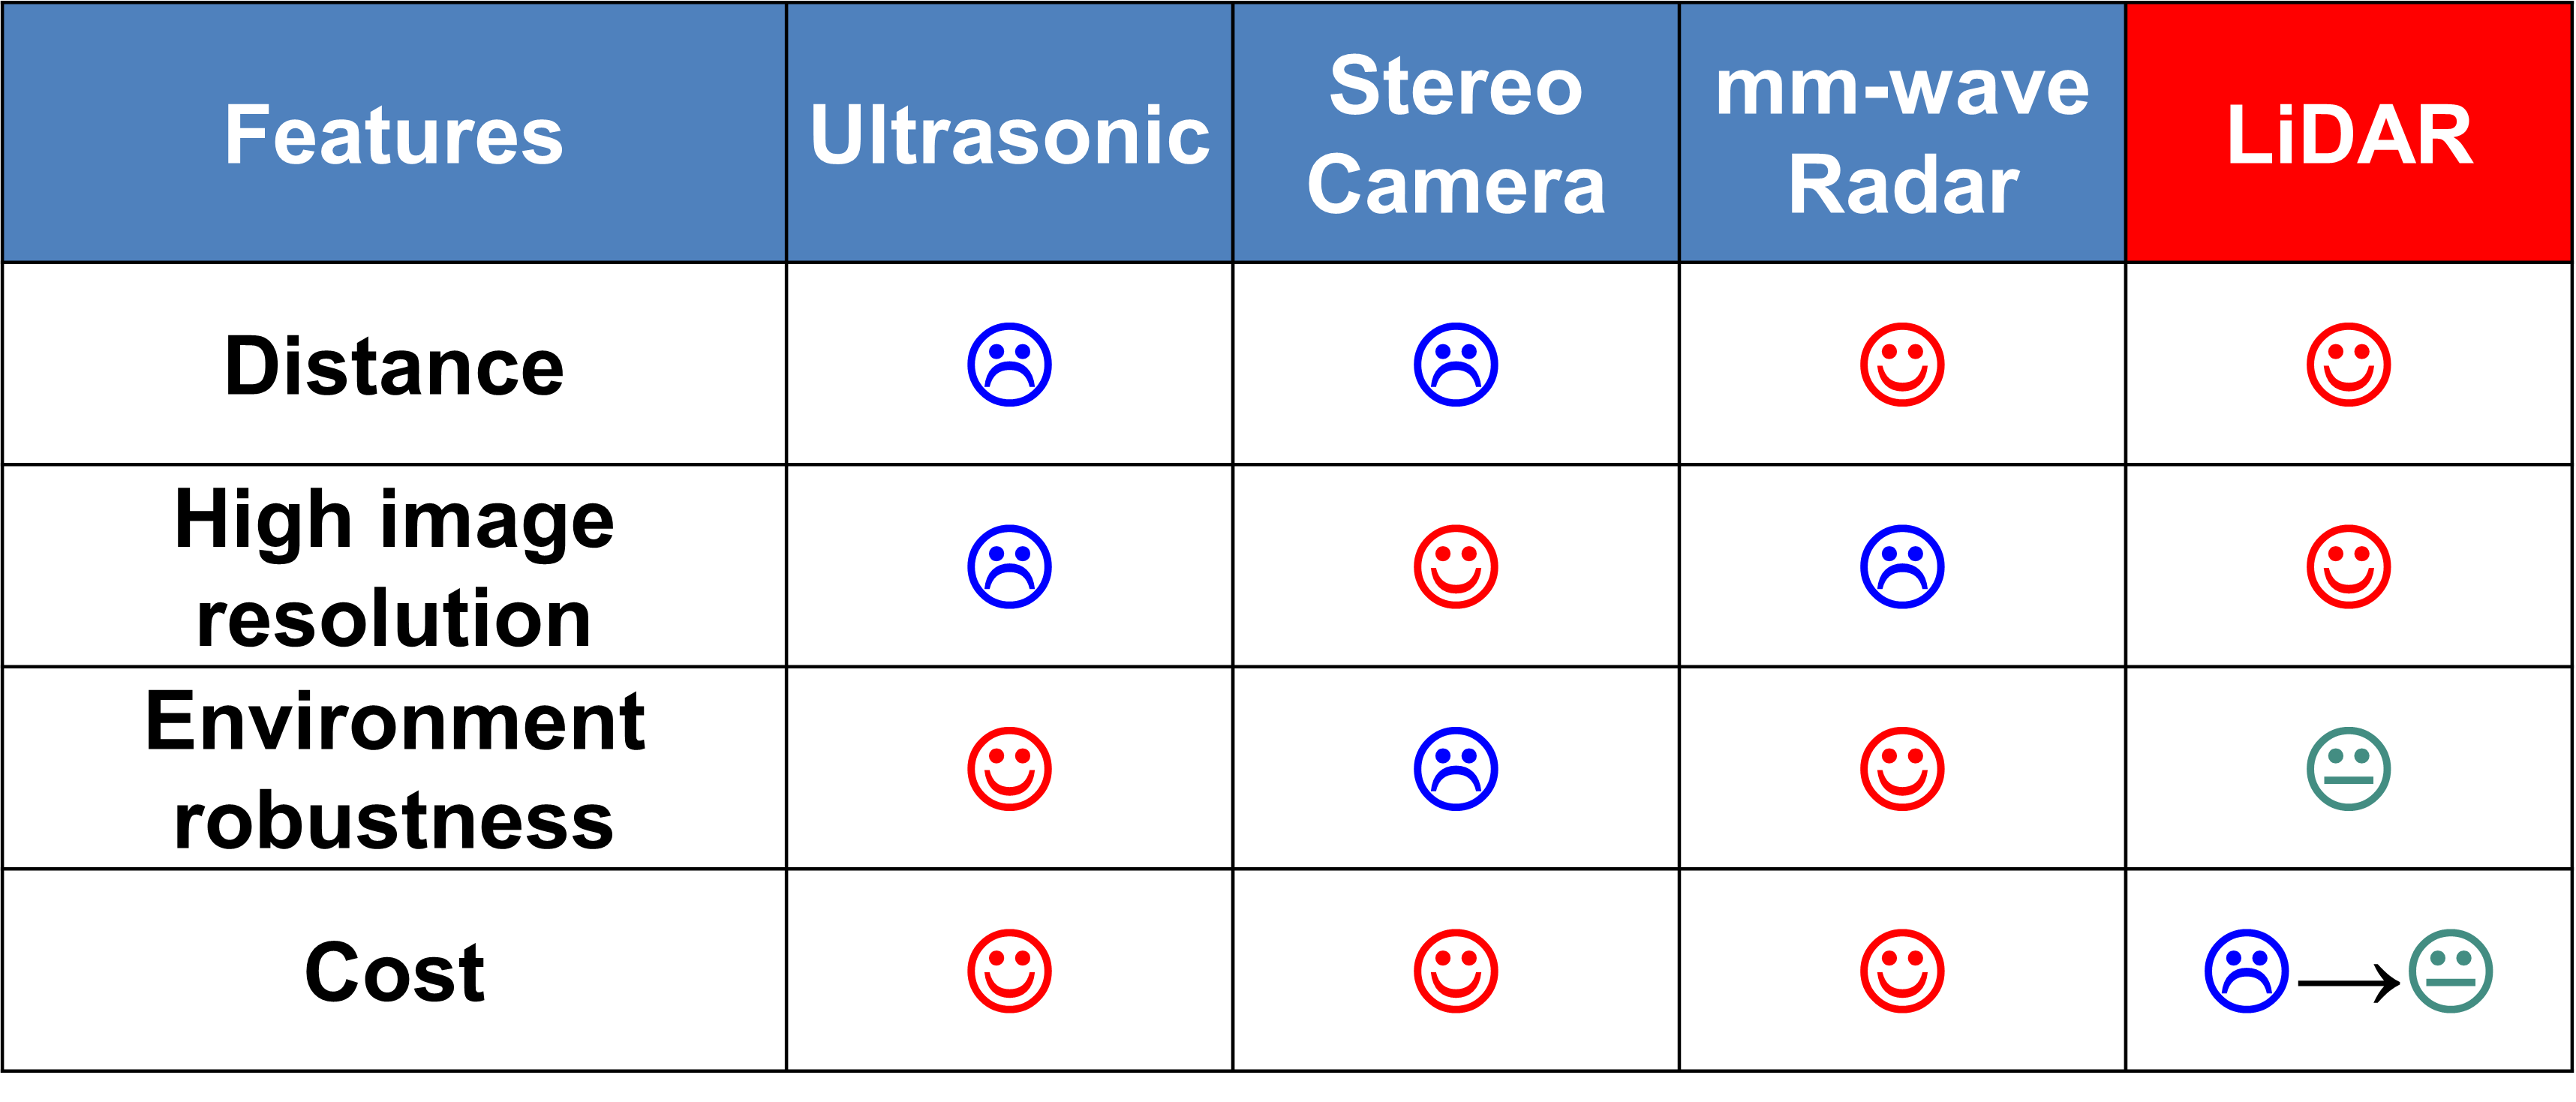
\includegraphics[width=0.5\textwidth]{figs/distancesensor.png}
\label{sensor}
\end{table}

We summarize the typical depth sensors used in ADAS systems in Table \ref{sensor}. It is important to note a trade-off between performance and cost for all sensors.
Unlike millimeter-wave (mmwave) radar, stereo cameras, and ultrasound sensors, LiDARs require a mechanical component for scanning, which makes LiDAR more expensive than other sensors. On the other hand, despite its cost, LiDARs have attracted attention because they are the only depth sensor that can provide high-resolution and long-range measurements.

Next, the requirements of the distance sensors for automated driving are discussed. Since 150m is the braking distance of a car travelling at 120km/h on a freeway, a distance sensor capable of sensing 200m is required for forward monitoring. This target is very challenging, regarding that the VLP-32\cite {velodyne} has a maximum distance of 50m and does not meet the requirements upon freeway use. Furthermore, when driving in urban areas, it is essential not to overlook pedestrians at a distance. Thus, depth-sensing with high-resolution is required (e.g. horizontal resolution of 0.1~0.2 degrees), which is very difficult to achieve with ultrasonic or radar sensors\cite{mitomo201077,lee2010fully}.

It is also crucial to have the capability to sense in all weather conditions (e.g. extreme sunlight, rain, snow, fog) to increase the reliability of automated driving. Among Table \ref{sensor}, the mmwave radar is a sensor that is not easily affected by the weather. On the other hand, when a LiDAR is placed in a foggy environment, its effective range is shortened because the laser is scattered. 
It is challenging to build a reliable automated driving system with a single sensor for these reasons. Thus, it will be necessary to take a sensor fusion approach where the sensors compensate for each other's weaknesses \cite{yeong2021sensor, loufusion}.

This paper reviews the development of automotive LiDAR for automatic driving from the aspect of circuit systems. Although a number of conference presentations have been made in recent years, to the best of the author's knowledge, there has been no comprehensive review paper on LiDARs for automatic driving.
The target readership of this paper is intended to be at the introductory level of ADAS LiDAR, and we set the goal to obtain a general overview of the research direction of the field. The main focus will be on dToF LiDAR with scanning mechanisms using 850-950nm lasers, which are expected to be mass-produced for automotive applications as of 2022 \cite{niclass2012100, niclass2008128, niclass20130, yoshioka201820, yoshioka201820ch, kondo2020automotive, ta20202d, akita2017imager, ito2013system, liu201960, kumagai2021189x600, ito2020back, seo2021direct, ouster}. 
Therefore, 1550nm LiDAR\cite{chung202119}, FMCW LiDAR\cite{behroozpour201611, poulton2017coherent}, Flash LiDAR\cite{ximenes2018256, padmanabhan20217, lindner2018252}, and iToF LiDAR\cite{kawahito2007cmos, bamji20140, bamji2018impixel, keel2019vga} are mentioned as comparisons but are not the main targets of the review. In addition, the discussion will focus as much as possible on the LiDAR circuit system, especially the photodetector (PD), readout circuitry, and signal processing, and the discussion of optics and lasers will be kept to a minimum.

We organize this paper as follows: in chapter 2, we explain the measurement principle of the dToF LiDAR and the issues unique to ADAS LiDARs. Then, in chapter 3, the first-generation LiDAR is studied in detail. While the first-generation LiDAR made a significant contribution to automated driving prototypes, its high cost held challenges to mass production. Next, in chapters 4 and 5, we will discuss how the latest LiDARs, which we call next-generation LiDARs, have made a breakthrough in cost and performance. Finally, chapter 6 summarizes and discusses the prospects of the field.

%%%%%%%%%%%%%%%%%%%%%%%%%%%%%%%%%%%%%%%%%%%%%%%%%%%%%%%%%%%%%
\section{LiDAR fundamentals}
\subsection{Automobile LiDAR challenges}
\begin{figure}[!t]
\centering
 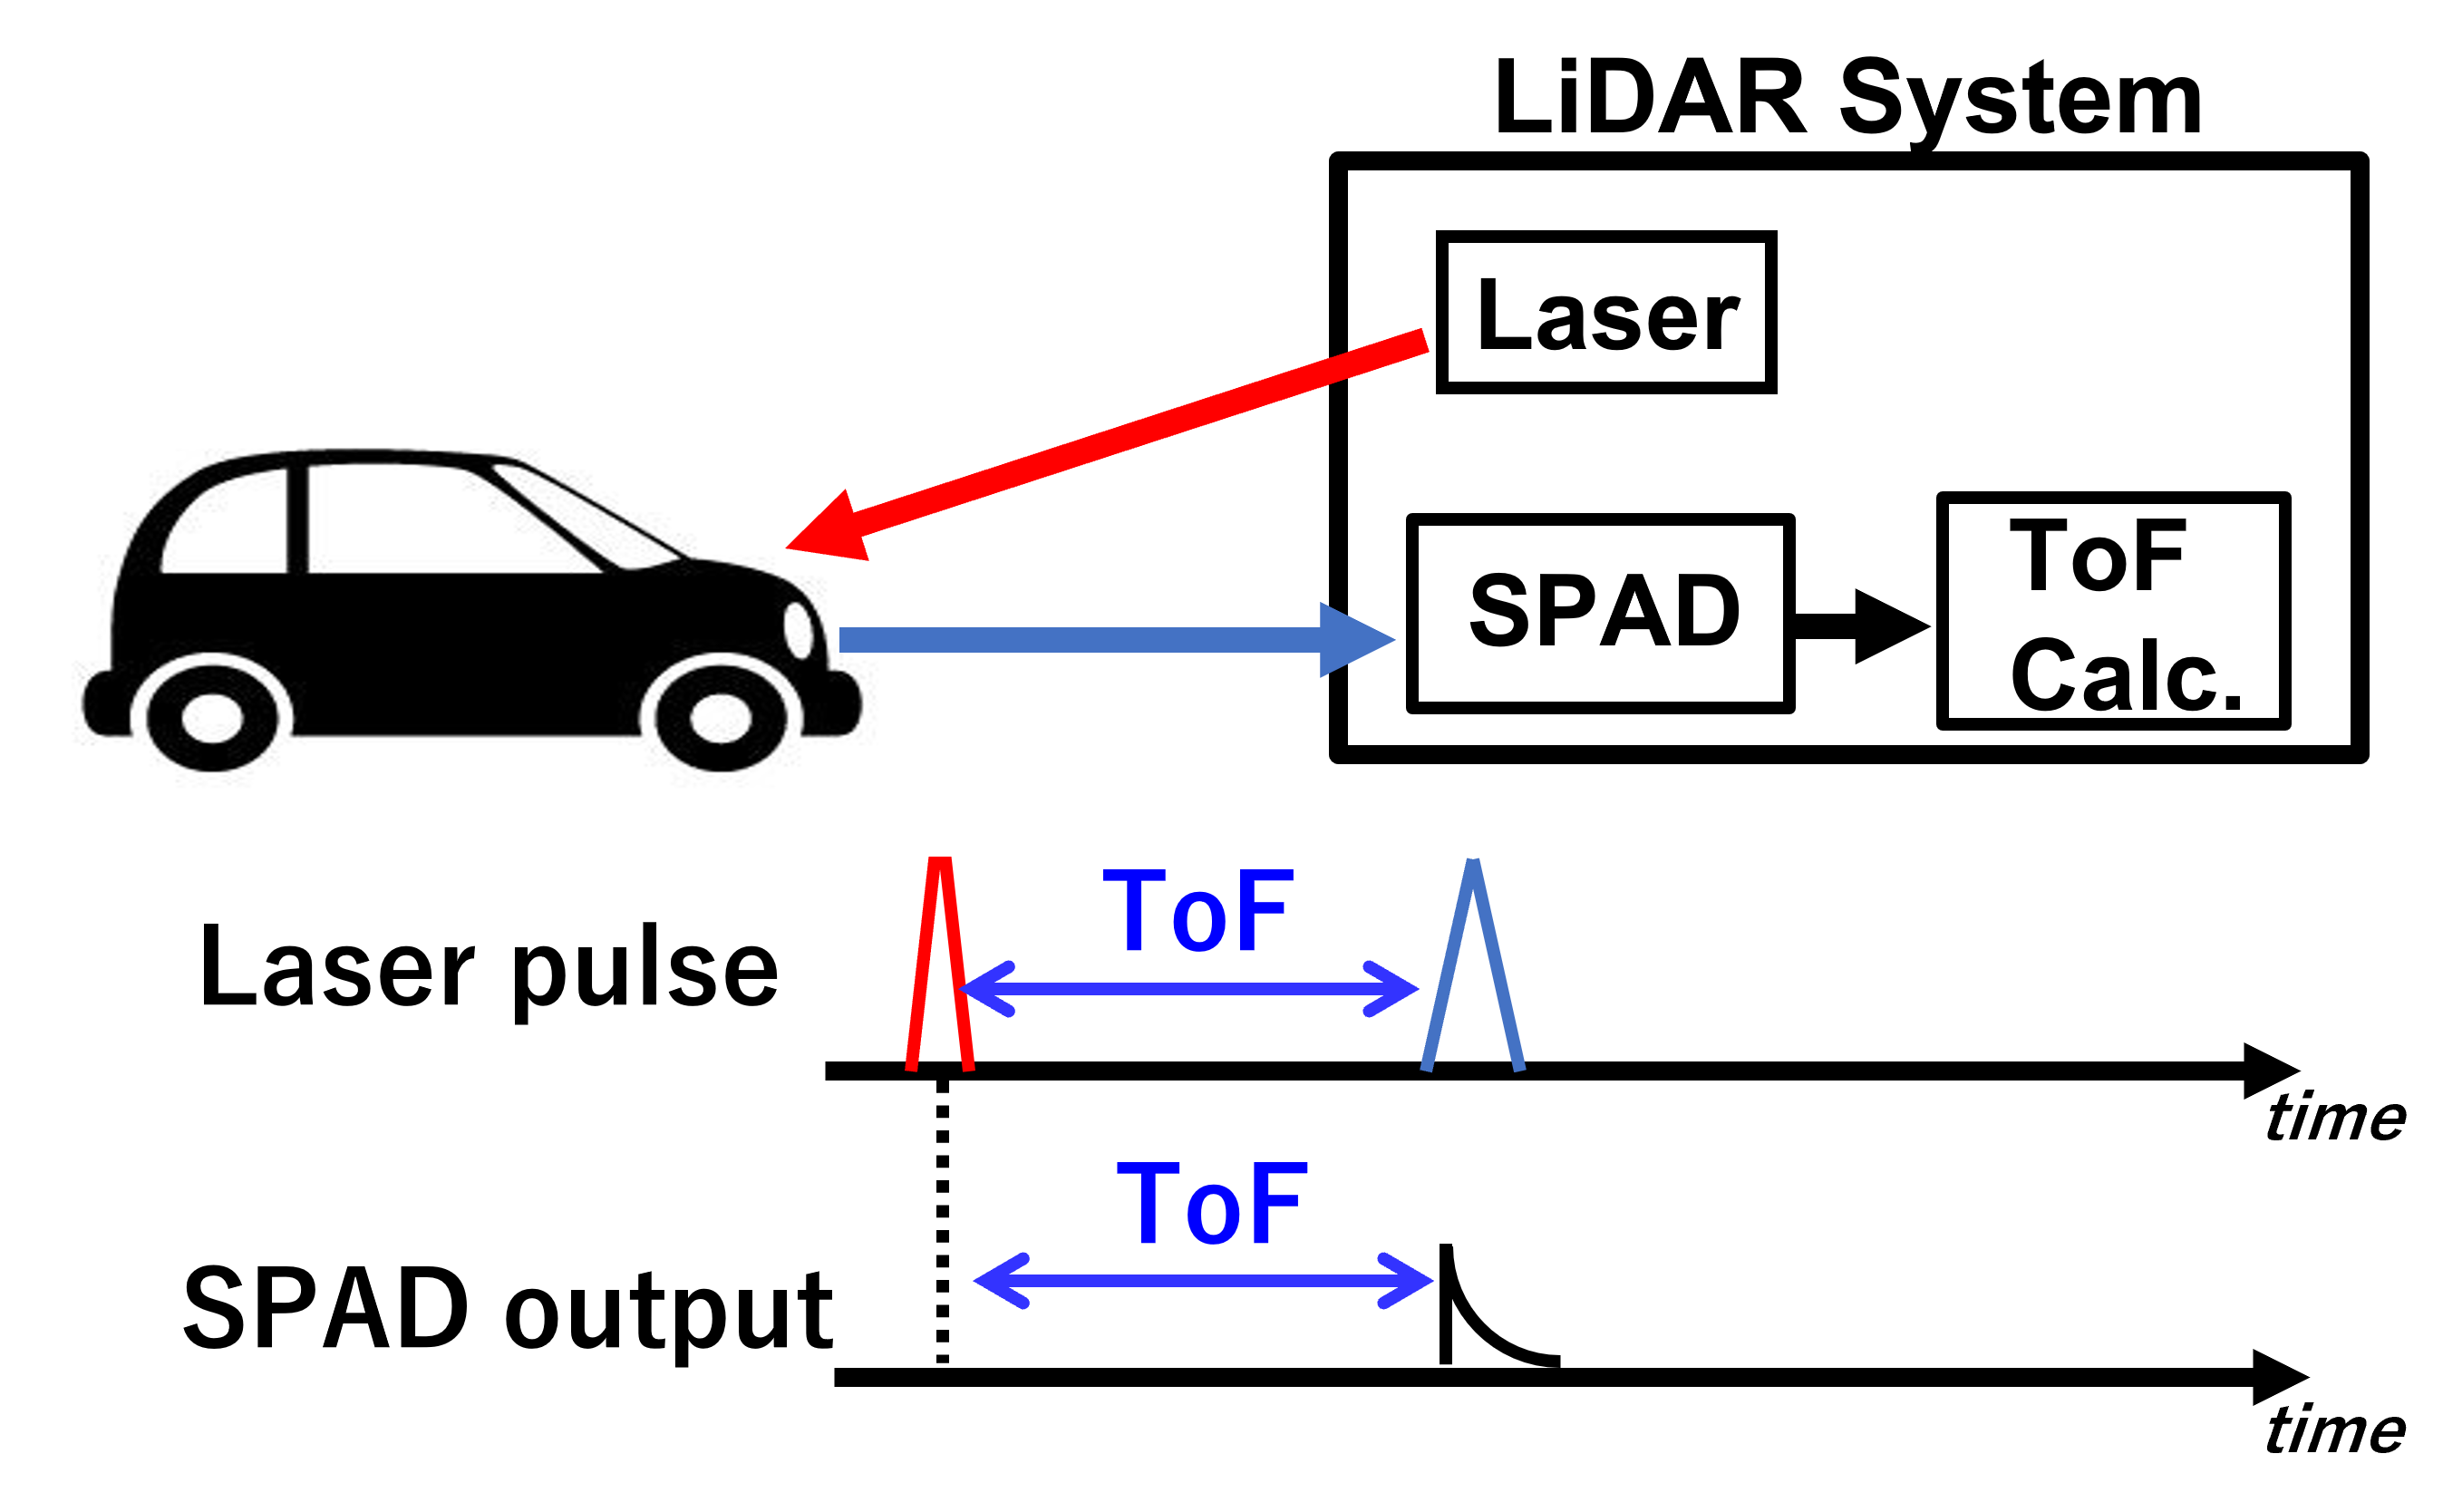
\includegraphics[width=0.49\textwidth]{figs/lidar.png}
  \caption{Distance measurement principle of dToF LiDARs.}
\label{lidar}
\end{figure}

\begin{figure}[!t]
\centering
 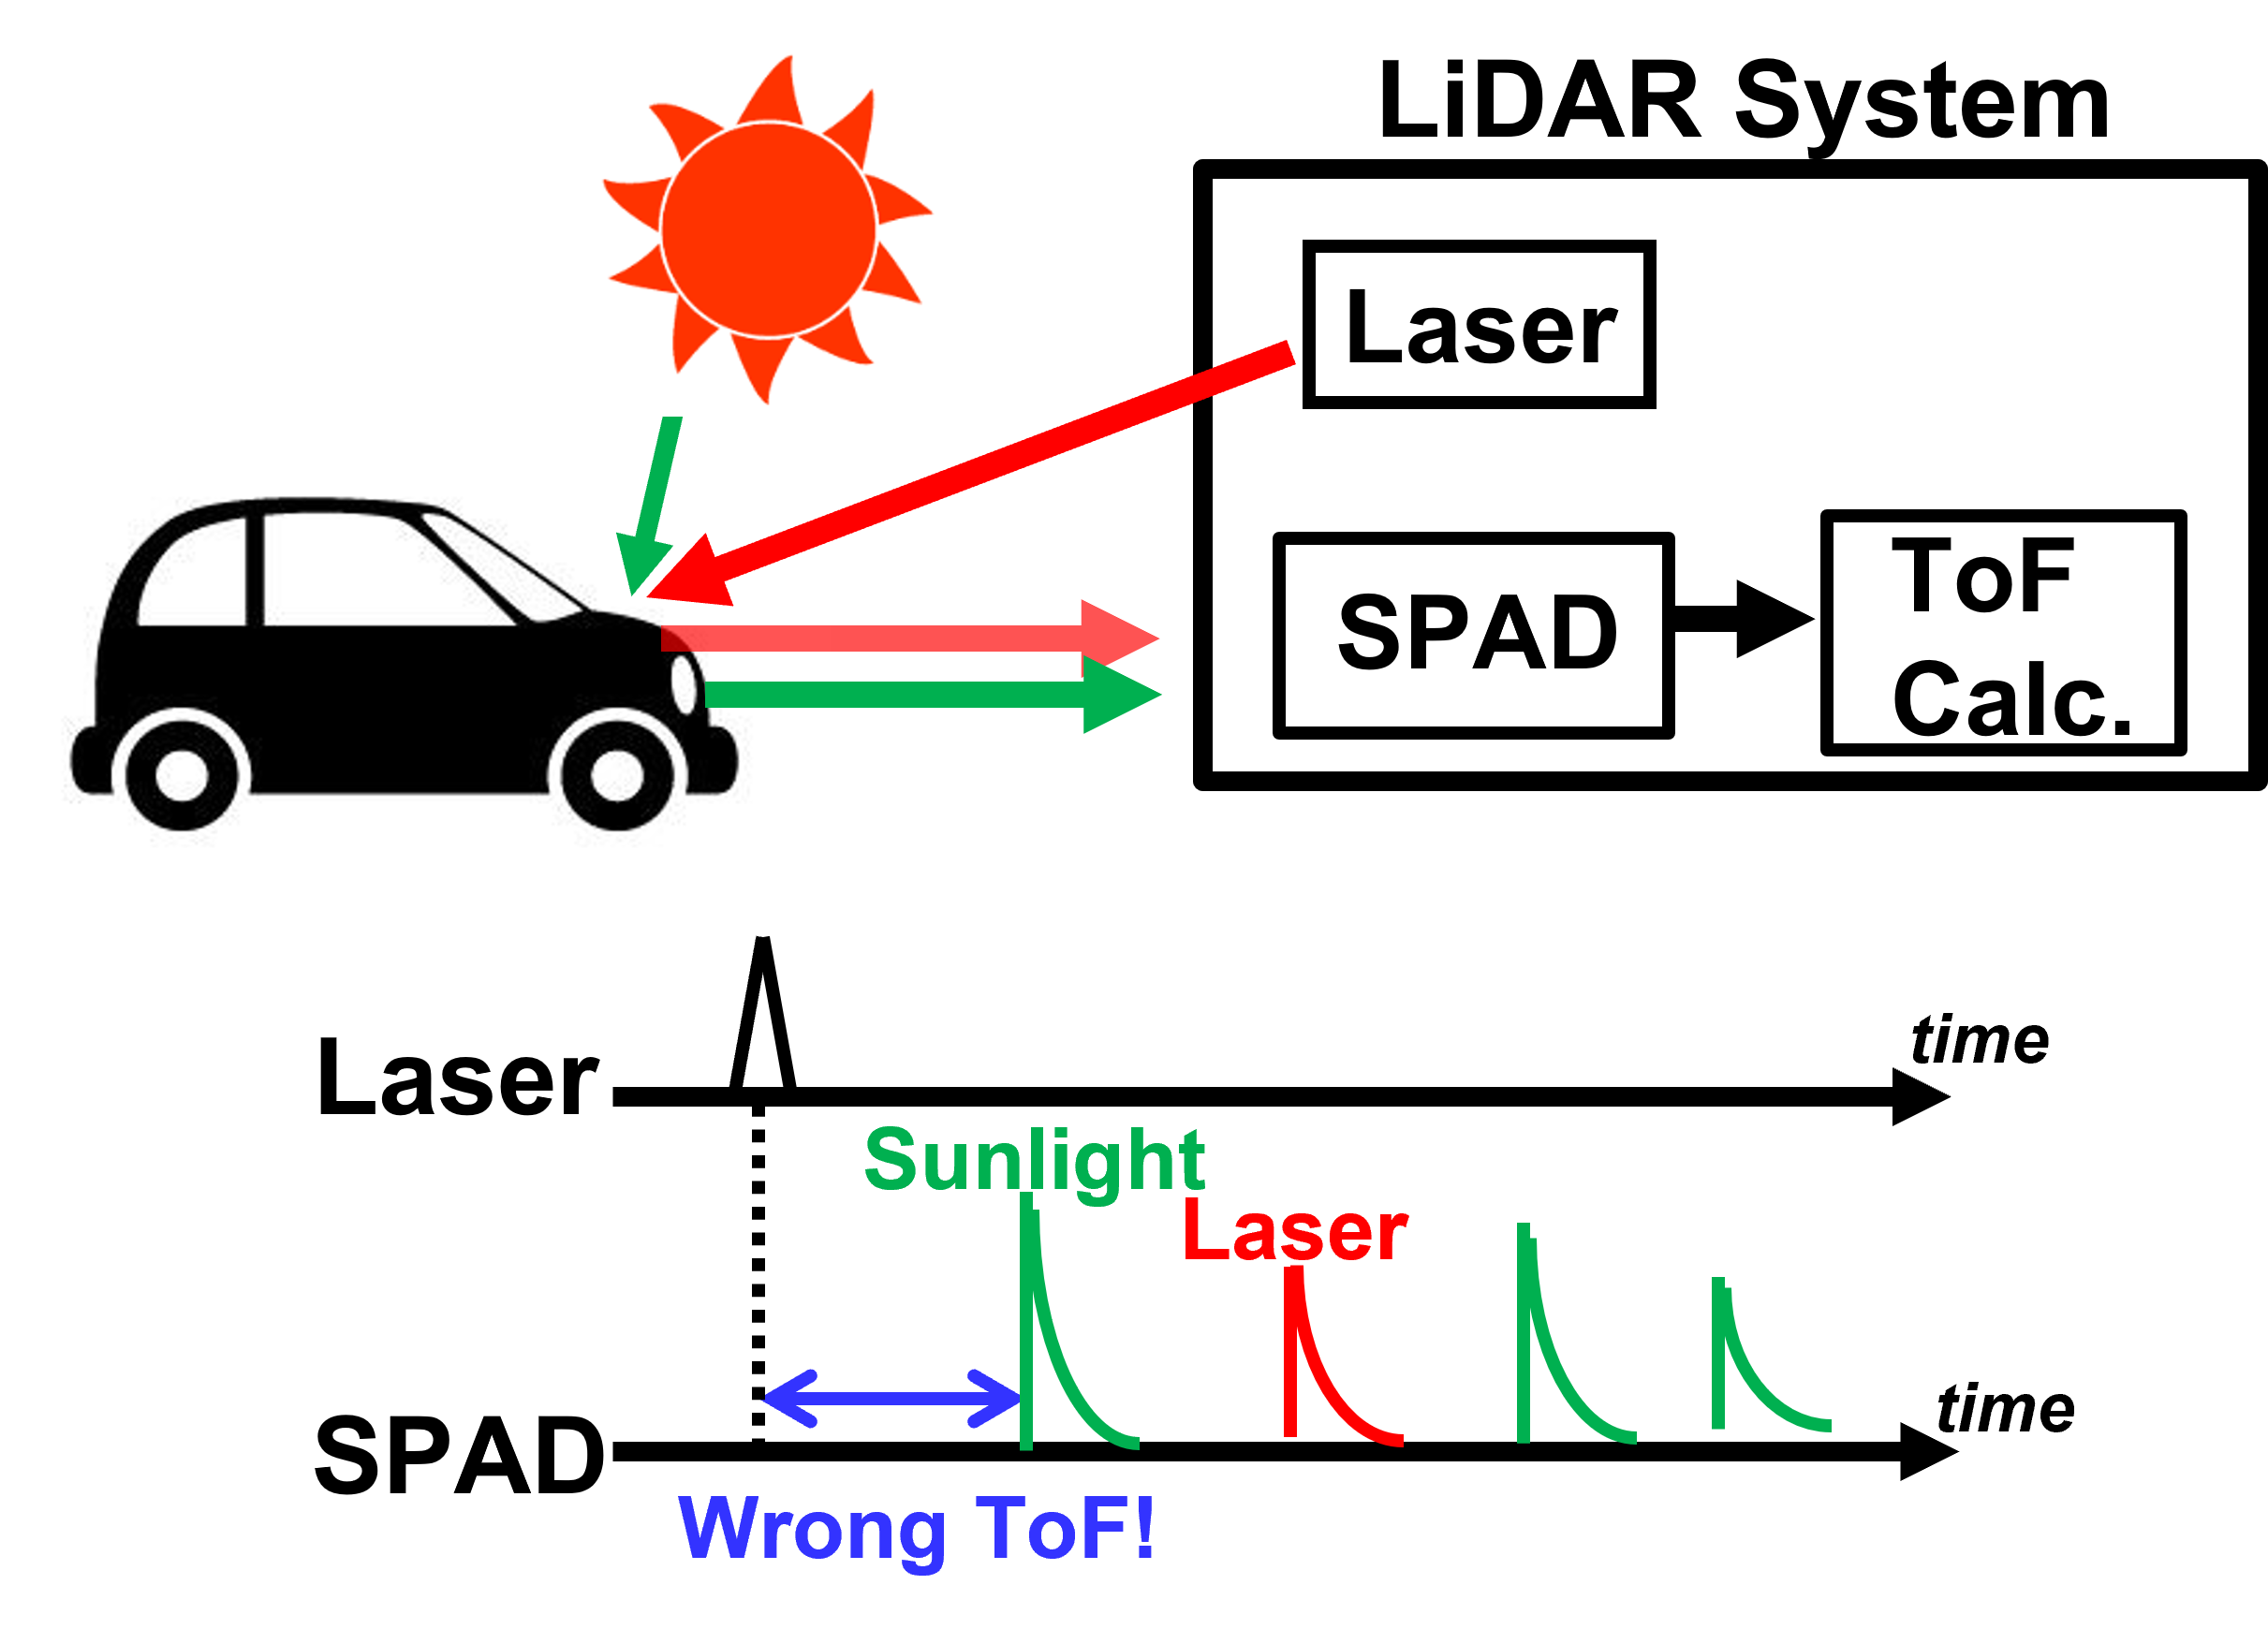
\includegraphics[width=0.49\textwidth]{figs/sunlight.png}
  \caption{In automotive LiDAR, strong sunlight is the biggest noise source and directly leads to measurement errors.}
\label{sunlight}
\end{figure}

\qquad First of all, the principle of direct Time of Flight (dToF) distance measurement is briefly explained based on Fig.\ref{lidar}. This type of LiDAR derives the distance based on the time-of-flight  (ToF), which is the time it takes for the laser emitted to reflect back from the target object.
\begin{eqnarray}
    \centering
    \textrm{Distance} = \frac{\textrm{Light speed} \times \textrm{ToF}}{2}
    \label{dist}
\end{eqnarray}
Thus, for accurate measurements, a readout circuit with high time resolution is required (e.g., ADC with a high sampling rate).

Although the dToF principle itself is simple, automotive LiDARs are difficult to design mainly because of the following points: 
\begin{itemize}
\item Since mounted on a fast-moving vehicle, long-range measurements are required.
\item For robust ADAS operation, it must provide accurate measurements despite various weather conditions.
\end{itemize}
For the former, the laser decays as the square of the distance. For example, the number of laser photons returned is 1/16 for 200m distance measurement compared to 50m, making the operation very difficult. Moreover, sunlight is the most significant noise source for outdoor LiDARs: for automotive applications, the LiDAR must function under extreme sunlight. Fig.\ref{sunlight} illustrates such harsh operating conditions, where the sunlight-triggered outputs can be larger than the laser in long-range measurement conditions.

In principle, LiDAR ranging can be expressed in terms of SNR, where the signal is defined as the number of returning laser photons and noise as the number of noise photons (mainly sunlight) input in a certain unit of time \cite{yoshioka201820}.
\begin{eqnarray}
    \centering
    \textrm{LiDAR SNR} = \log_{20}{\frac{\textrm{Number of laser photons}}{\textrm{Number of noise photons}}}
    \label{snr}
\end{eqnarray}
Another restriction for automotive LiDAR is that the emitting laser power must comply with eye safety requirements. For automotive applications, it is common to comply with the strictest class-1 eye safety, i.e., the laser must not harm the human eye under any circumstances. In other words, due to the strict laser power limitations, the signal power cannot be further increased. On the other hand, eq.(\ref{snr}) shows that optical filters that filter sunlight and increased sensitivity of PDs can contribute to SNR.

%(SNRを帰ってくるフォトン数と捉えると反射率、光学系、レーザパワー、受光素子感度、スキャン機構、FPS、解像度の複雑な関数となる。そのためLiDAR研究間で直接性能比較をすることは非常に難しくどの研究の性能が一概に良いとは一言で言えない。例えばMEMSを採用しているLiDARでは論文では直接比較できないコストや筐体体積といったファクターで優れる反面、内部MEMSミラーにおけるロスが大きいためSNRは悪化してしまい達成可能な最大距離は低下してしまう。)

\subsection{Basic LiDAR architectures}
\begin{figure}[!t]
\centering
 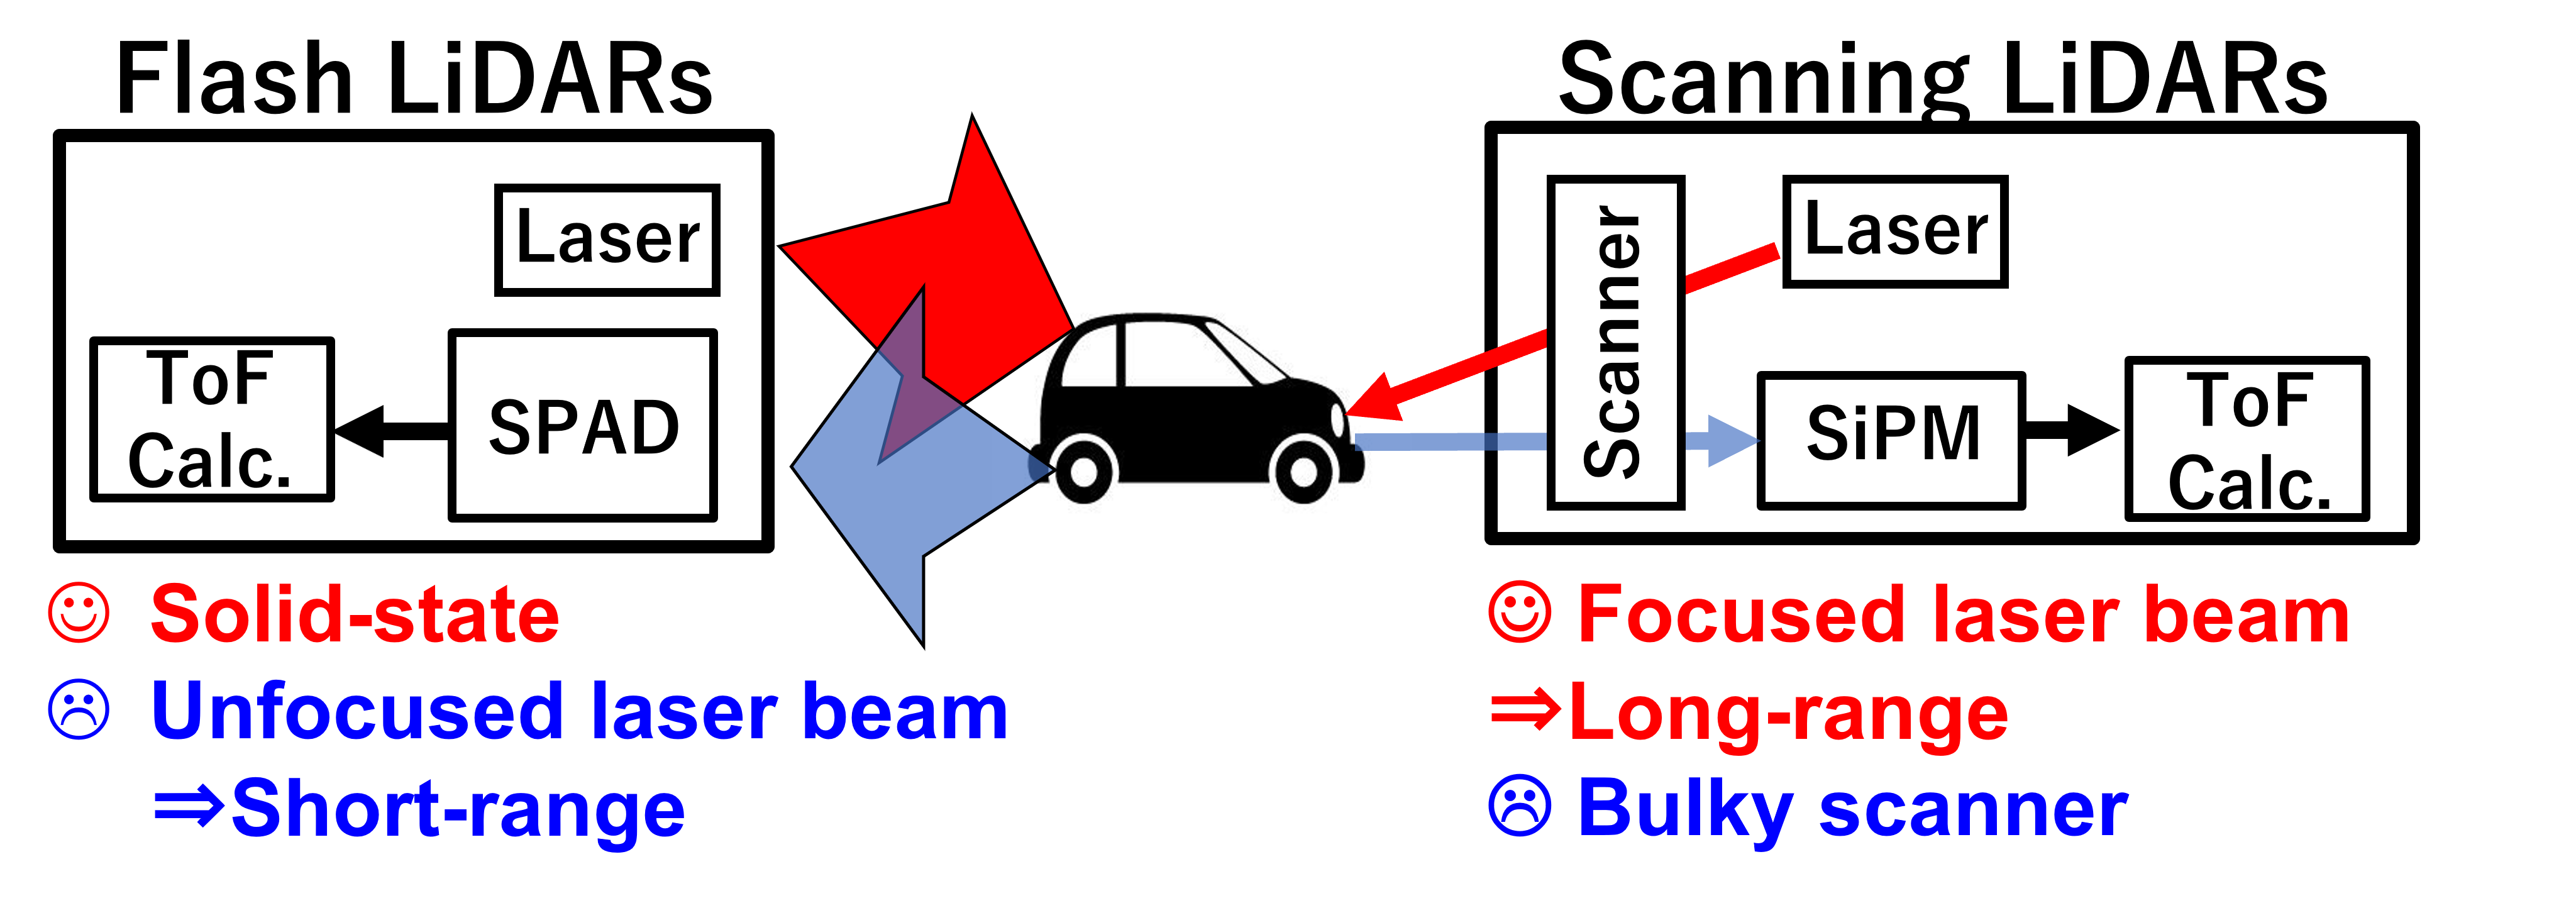
\includegraphics[width=0.49\textwidth]{figs/flashscan.png}
  \caption{A comparison between flash-type LiDAR and scan-type LiDAR is shown. Flash-type LiDAR irradiates the laser beam over the entire FoV at once, while scan-type LiDAR utilizes a scanning mechanism to scan the laser beam in order. On the other hand, the SNR is high for the latter because the laser power can be concentrated in a small number of pixels, and such scanning is essential for long-distance measurements such as 200m.}
\label{flash}
\end{figure}

\qquad The operating principle of Fig.\ref{lidar} is referred to as direct ToF (dToF), which is the mainstream method for automotive LiDAR. On the other hand, the indirect ToF (iToF) method modulates the laser and measures the distance by detecting the phase shift and enables higher precision \cite{kawahito2007cmos, bamji20140, bamji2018impixel, keel2019vga}. However, iToF holds a trade-off between measurement distance and accuracy, since higher sensor modulation frequency leads to precise measurement but shorter measurement distances. In addition, since the photodetector must have a linear response to capture the modulated laser, it is necessary to use an avalanche photodiode (APD) instead of a highly sensitive single-photon avalanche diode (SPAD). As a result, the PD sensitivity is inevitably lower than that of the dToF method. For these two reasons, it is challenging to achieve the 200m measurement performance required for ADAS, and iToF may be more suited for short-range applications requiring high precision, such as robotics\cite{yoshioka2021through}.

\begin{figure}[!t]
\centering
 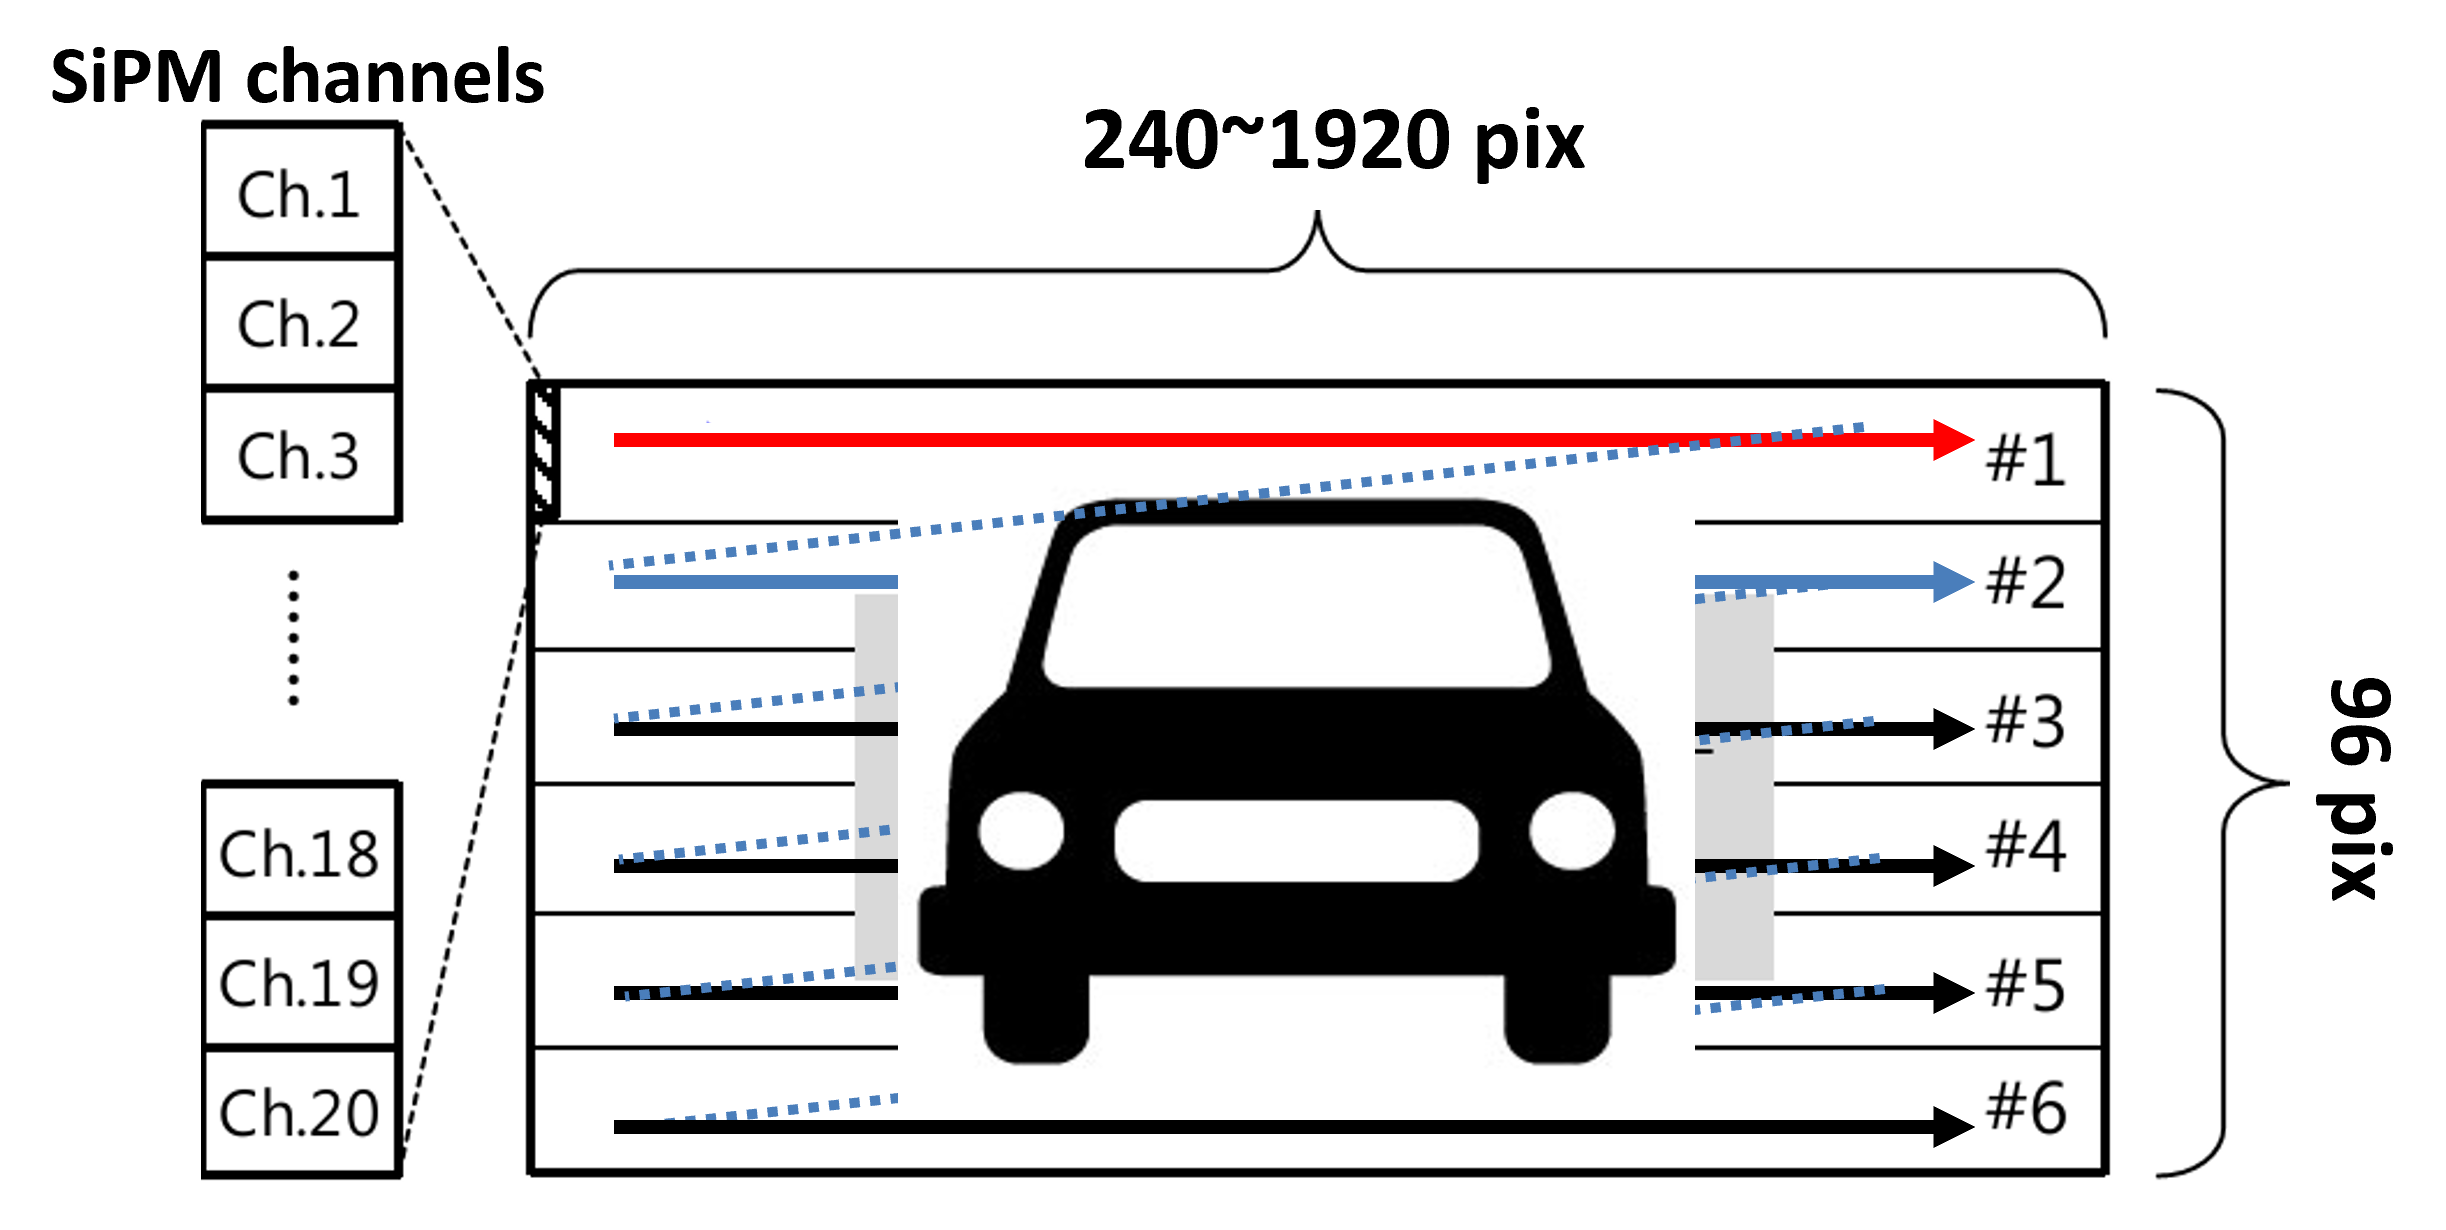
\includegraphics[width=0.5 \textwidth]{figs/raster.png}
  \caption{A diagram showing a raster scanning LiDAR system. Typically, 2D raster scanning requires scanning mechanisms for both the laser (TX) and the returning laser (RX) paths.}
\label{raster}
\end{figure}

The dToF LiDARs can be categorized into two types: flash \cite{ximenes2018256, padmanabhan20217, lindner2018252} and scanning. As shown in Fig.\ref{flash}, the flash emits a laser beam over the entire field of view, and a 2D array of PDs receives the reflected light, similar to image sensors. The advantage of the flash method is that the LiDAR is free of mechanical parts, resulting in a low cost and a high frame rate. However, when the number of pixels in the flash LiDAR is $N \times M$, the laser power $P$ will be diffused to $N \times M$ pixels, which result in a weak laser power of $P/(N \times M)$ per pixel. Therefore, while high resolution is easy to achieve with flash LiDARs, long-distance measurement such as $>$20m is difficult. Therefore, the flash LiDAR's potential applications are short-range LiDARs attached to the side of a car or robotics application. On the other hand, the scanning LiDARs obtain $M$ pixels and conduct a horizontal/vertical scan. Thus, the laser power per pixel is $P/M$, which is much better than the flash. On the other hand, the cost and frame rates degrade due to the scanning procedure.

There are also several types of LiDAR scanning methods: rotating mirror\cite{velodyne,ouster}, polygon mirror\cite{niclass2012100,yoshioka201820,kondo2020automotive}, and MEMS mirror \cite{ito2013system, akita2017imager, kumagai2021189x600}.  The rotating mirror is extremely bulky but generally has good optical properties (less laser attenuation) and can obtain 360-degree data.
The polygon mirror obtains data by raster scanning within the FoV, as shown in Fig.\ref{raster}. In order to perform such scans, two actuating mirrors are utilized for both the laser and the receiver optical path. Thus, the implementation becomes bulky, due to the installment of the mirror itself and the motor driving the mirror.
Finally, the MEMS mirror eliminates the need for bulky mechanical components by using an extreamly small movable micro-mirror. Therefore, the size of the LiDAR can be significantly reduced and is sometimes referred to as solid-state LiDAR. On the other hand, the MEMS mirror has poor optical properties; the trade-off is the degradation in LiDAR SNR.

%%%%%%%%%%%%%%%%%%%%%%%%%%%%%%%%%%%%%%%%%%%%%%%%%%%%%%%%%%%%%%%%%%%%%%%%%%%%%%%%
\section{First Generation LiDARs}
\begin{figure}[!t]
\centering
 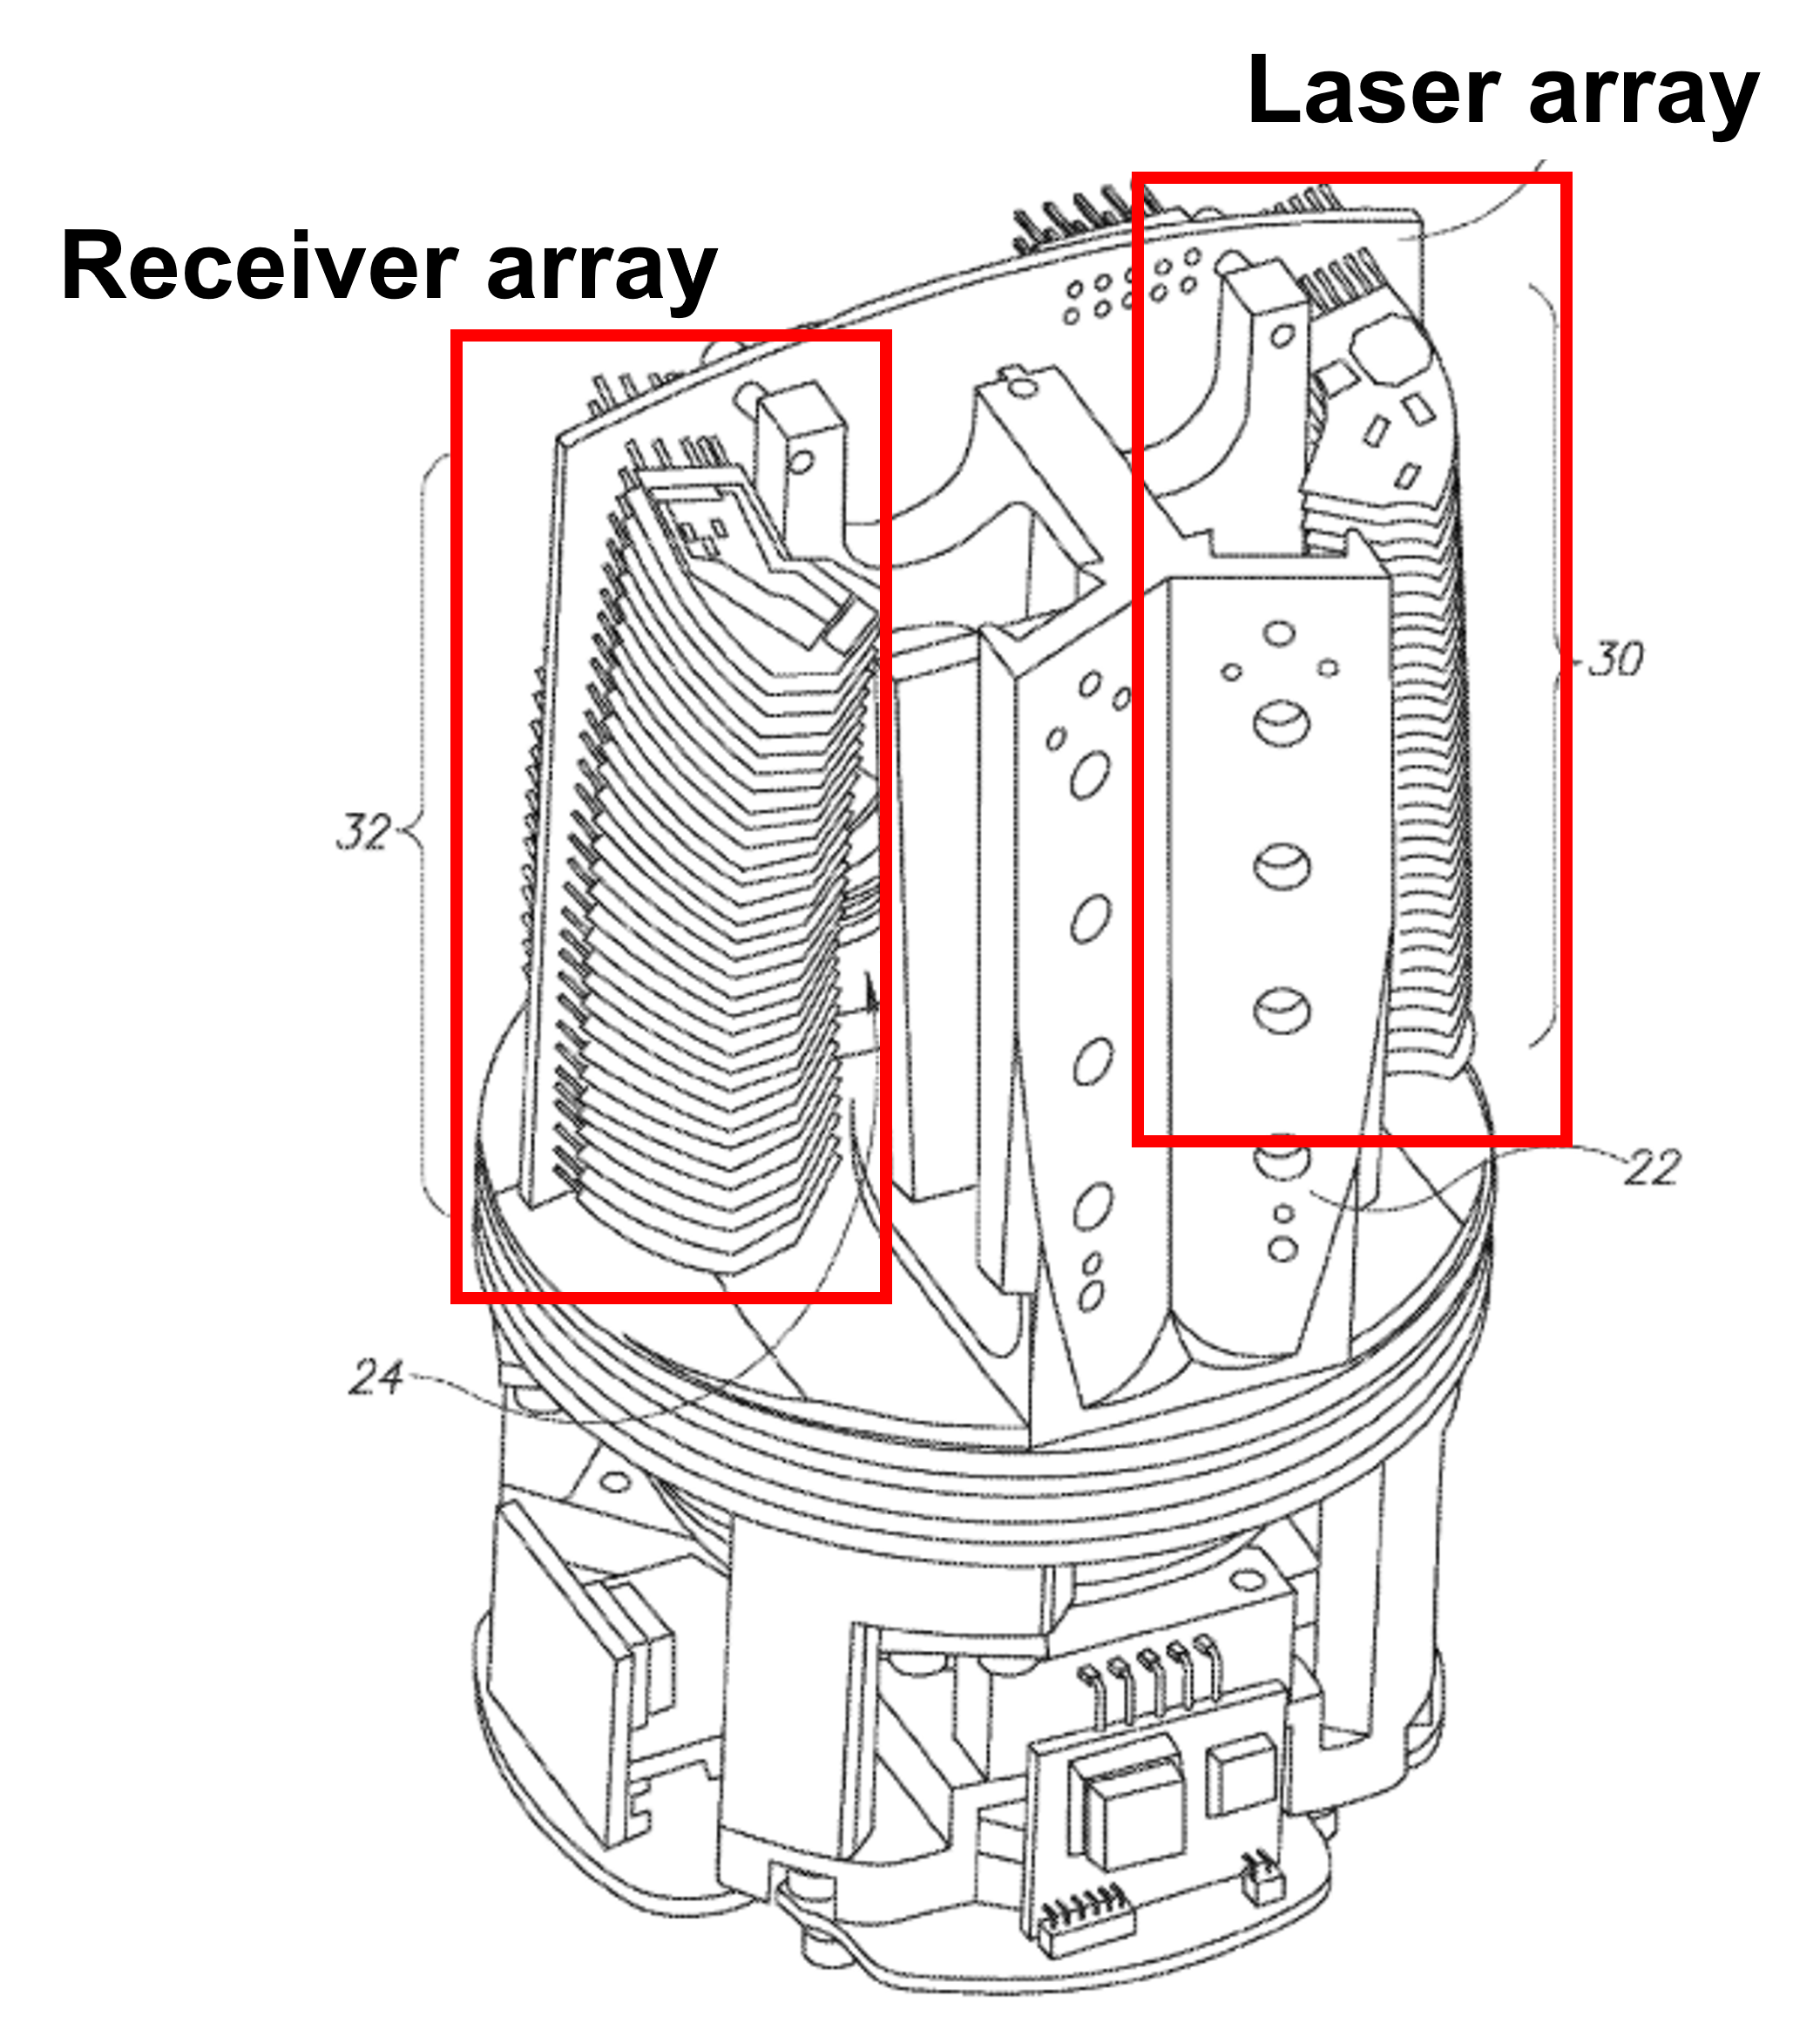
\includegraphics[width=0.39\textwidth]{figs/velo.png}
  \caption{Velodyne HDL-32 diagram \cite{velopatent}}
\label{velo}
\end{figure}

\qquad Velodyne's rotational LiDAR\cite{velodyne, velopatent}, shown in Fig.\ref{velo}, is implemented by stacking the laser and receiver boards vertically.
We define such LiDAR as the \textit{first generation LiDAR} in this paper, as it was released at the infancy of ADAS LiDAR. Nevertheless, such LiDARs realized high-quality depth sensing and played a key role in many self-driving prototypes \cite{montemerlo2008junior}.

As shown in the schematic in Fig.\ref{next}(a), the APD is used as the PD of the first-generation LIDAR. The APD output is amplified by TIA and VGA and then quantized by a high-speed ADC, and the ToF was calculated in the digital processor.
The first generation LIDAR can be seen as an integration of "point" measuring distance sensors consisting of a laser and PD pair.
On the other hand, such implementation required many discrete components. As a result, the cost of the first generation LiDAR was very high and fragile. In addition, it was difficult to scale the performance on the same body because the increase in resolution directly impacted the number of components. Moreover, although APDs are more sensitive than ordinary photodetectors, they were inadequate for long-distance measurements.

%%%%%%%%%%%%%%%%%%%%%%%%%%%%%%%%%%%%%%%%%%%%%%%%%%%%%%%%%%%%%%%%%%%%%%%%%%%%%%%%
\section{Next Generation LiDARs}
\begin{figure*}[!t]
\centering
 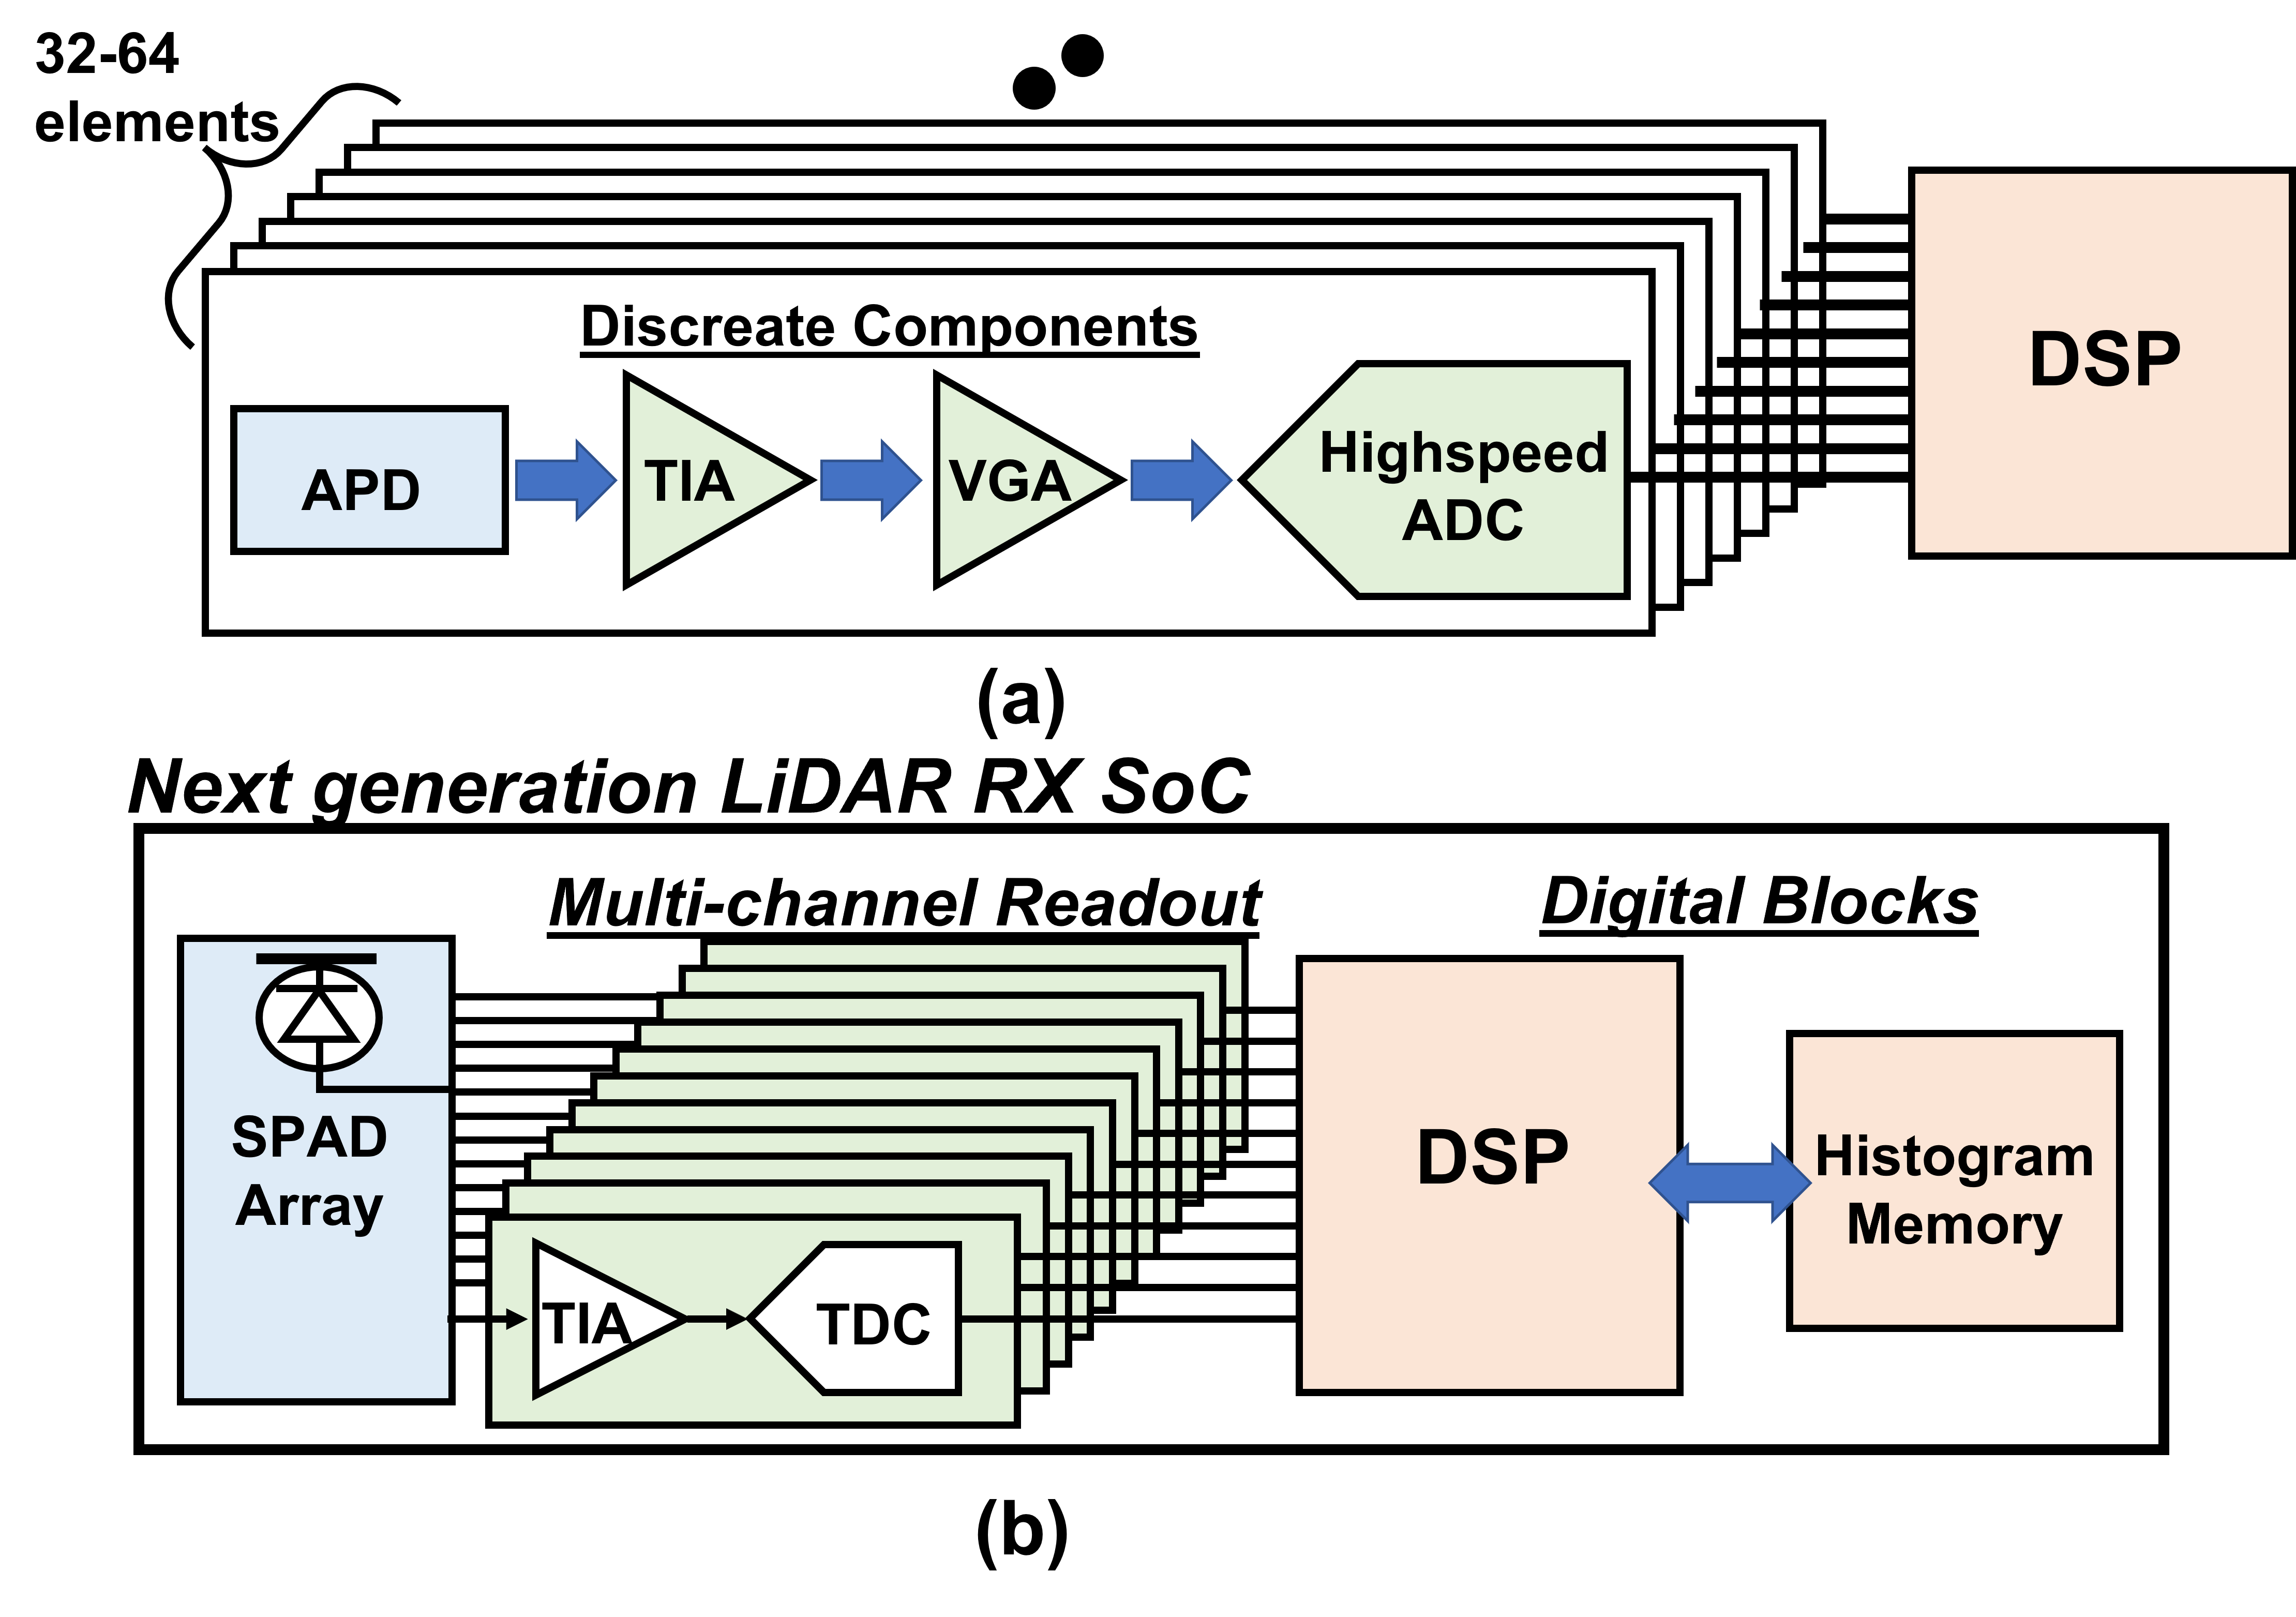
\includegraphics[width=0.75\textwidth]{figs/nextlidar.png}
  \caption{(a) System diagram of first-generation LiDAR. (b) System diagram of next-generation LiDARs.}
\label{next}
\end{figure*}

\begin{figure}[!t]
\centering
 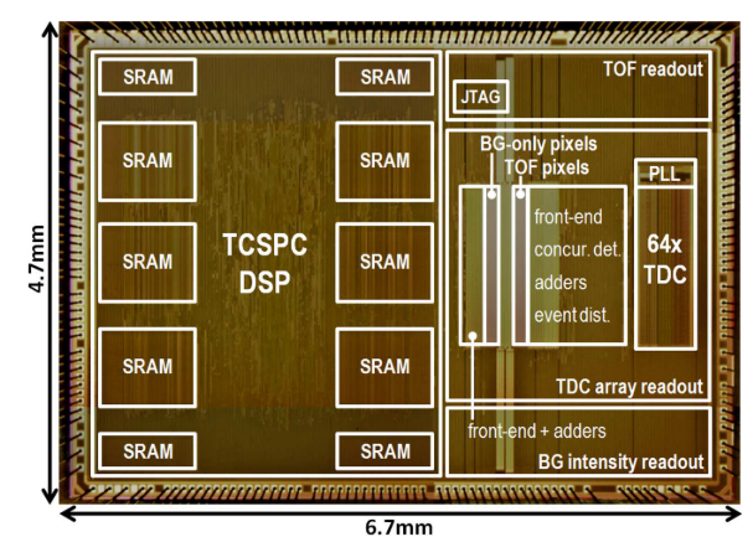
\includegraphics[width=0.4\textwidth]{figs/niclasschip.png}
  \caption{Fully integrated LiDAR SoC \cite{niclass2012100}}
\label{chip}
\end{figure}

\qquad The first-generation LiDAR advanced the horizon of automated driving and greatly expanded the ADAS market. However, it was challenging to adopt this technology in mass-produced vehicles without lowering costs and extending its performance. 
To achieve these goals, research on \textit{next-generation LiDAR} has been carried out.
In this paper, we discuss the fundamental concept of the next-generation LiDAR as \textbf{the integration of SPAD, readout circuit, and the signal processing circuit}.

Illustrated in Fig.\ref{next}(b), ref.\cite{niclass2012100} is a breakthrough in LiDAR SoC, which achieves the integration of the SPAD array, readout circuit, DSP and memory in a single chip. For automotive LiDAR, the number of SPADs per pixel is several 10s to mitigate the quenching time as described below. As a result, the total number of SPADs in the array is in the order of 100-1000. Thus, connecting these SPADs to the signal processing circuit is quite challenging. Therefore, ref.\cite{niclass2012100} designed a SoC using a high voltage CMOS process to integrate 384 SPADs, readout circuits, DSPs, and memory on a single chip.

In contrast to the first-generation LiDARs that used many discrete components, this SoC achieves the same function on a single chip, paving the way for significantly low-cost LiDARs. In addition, as is known as Moore's Law, CMOS scaling is expected to increase the number of transistors with a lower cost, making the LiDAR performance scalable.

\subsection{SPAD detectors}
\begin{figure}[!t]
\centering
 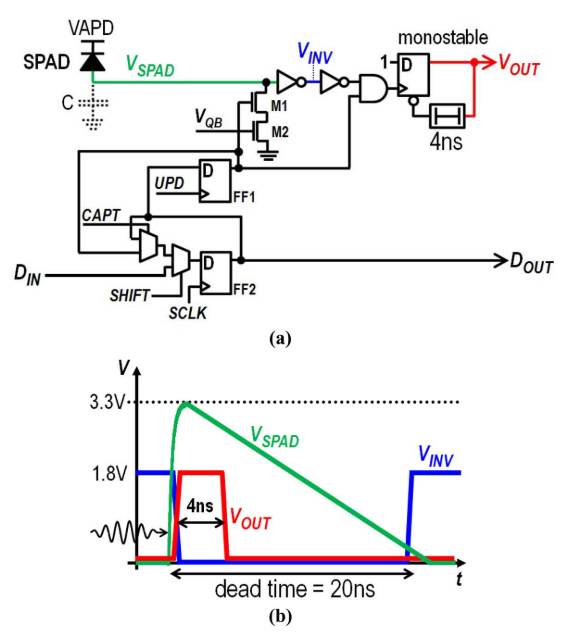
\includegraphics[width=0.4\textwidth]{figs/spad.png}
  \caption{Schematic of SPAD with passive quenching \cite{niclass2007spad}}
\label{spad}
\end{figure}

\qquad Both APDs and SPADs operate photodiodes with a strong reverse bias, but SPADs are very sensitive photodetectors capable of single-photon detection \cite{niclass2005design, zappa2007spad, stoppa2009spad, niclass2007spad, gariepy2015single}. SPADs are biased above the breakdown voltage (20-30V in silicon) to operate the diodes in the Geiger mode. In Geiger mode, when a photon is received, the amplification ratio of the device ideally becomes infinite, allowing the detection of single photons by flowing a large current independent of the photon intensity. On the other hand, if such a current continues to flow, the device will be destroyed. Therefore, negative feedback is applied by the accompanying quenching resistor to stop the current forcibly as in Fig.\ref{spad}.

The SPAD contributes to the long-range performance of the LiDAR because its strong amplification enables the detection of single photon and faint returning lasers during long distance measurements. The key SPAD design parameter is the photon receiving probability and directly relates to device sensitivity (i.e. quantum efficiency or photon detection efficiency (PDE)). The other parameters are the quenching time and the number of SPADs assigned to each pixel. The higher the PDE, weaker lasers can be detected, directly affecting long-distance performance. In addition, the quenching time is closely related to sunlight resistance. If the quenching time is long, pile-up occurs when the SPAD cannot respond to the laser after it is ignited by noise light such as sunlight. The best way to reduce the quenching time is to lower the quenching resistance, but this is typically a trade-off against device reliability. In general, multiple SPADs are utilized in each pixel to mitigate the pile-up by providing redundancy. Even if one SPAD fires, another SPAD can receive the laser signal.

\subsection{TDC based readout circuitry}
\qquad While the output of an APD is an analog quantity proportional to the intensity of light,  SPAD output can be treated as a digital pulse by shaping the output with a buffer (as in Fig.\ref{spad} $V_{out}$). Moreover, dToF LiDARs can sufficiently calculate the ToF from the time between the laser emission and the pulse rise. In addition, while it is difficult to implement several tens or hundreds of high-speed ADCs on an SoC due to its small area, a time-to-digital converter (TDC) circuit is used in \cite{niclass2012100}, which is a circuit specialized to measure time. TDC was initially introduced as a time quantization circuit for digital PLLs and returns the digital value of the time difference between the two inputs \cite{leetdc, elkholytdc}.
Compared to ADCs, TDCs can be composed almost out of digital circuits, and by distributing the reference clock signal to a large number of TDCs, an array of TDCs can be realized with a small area. In addition, the available time resolution of TDCs is as high as 10-100 ps, achieving ToF accuracy that cannot be easily achieved with ADCs.

\subsection{Signal processing circuits}
\begin{figure}[!t]
\centering
 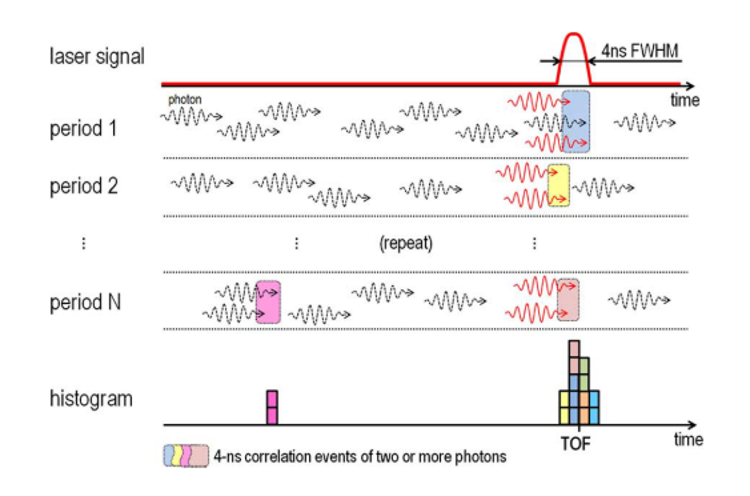
\includegraphics[width=0.5\textwidth]{figs/threshold.png}
  \caption{TDC readout mechanism in \cite{niclass2012100}}
\label{tdc}
\end{figure}

%\begin{figure}[!t]
%\centering
% 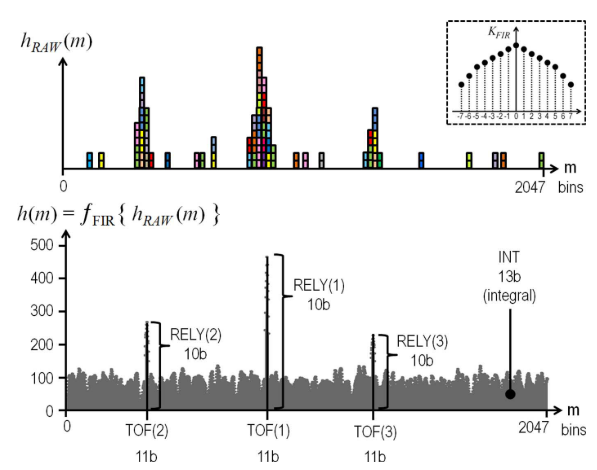
\includegraphics[width=0.5\textwidth]{figs/hist.png}
%  \caption{Histogramming and FIR filtering method utilized in \cite{niclass2012100}}
%\label{hist}
%\end{figure}

\begin{figure}[!t]
\centering
 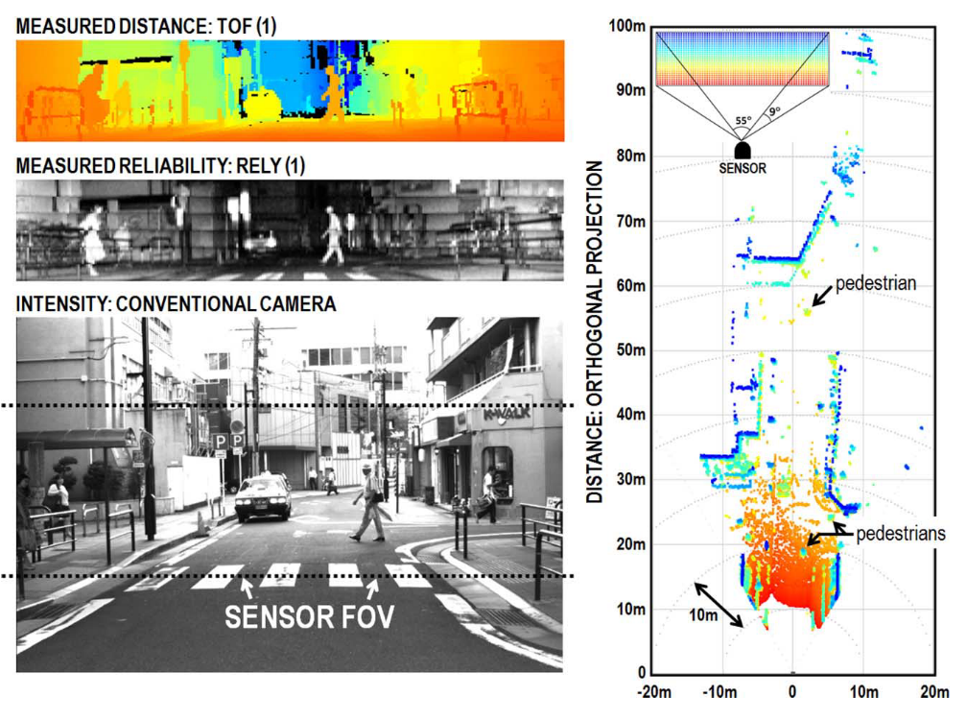
\includegraphics[width=0.5\textwidth]{figs/distance_image.png}
  \caption{Measurement result of \cite{niclass2012100}. Thanks to the one-chip integration and rich signal processing, the lidar achieves distance performance of 100m.}
\label{meas}
\end{figure}

\qquad The SoC integration made room for a richer signal processing, leading to the development of signal processing techniques specific to dToF LiDAR. One of the most popular signal processing methods is signal accumulation. As shown in Fig.\ref{tdc}, by accumulating the $N$ TDC measurement results in the same situation and obtaining a histogram, the accumulation can improve the SNR by $\sqrt{N}$. While sunlight is a random event with no correlation, laser light is a deterministic event and is observed at the same time. By using accumulation, the SNR improves as the number of measurements is increased, but it is a tradeoff with FPS since it takes more measurements to obtain a single pixel.

In addition, in \cite{niclass2012100}, a certain threshold for TDC activation is used to increase sunlight tolerance.
The problems caused by sunlight are: 1) the histogram memory become gigantic if all incoming sunlight events are recorded, 2) due to the finite TDC reset time, the TDC may miss the laser if the sunlight triggers the TDC. Therefore, by adding a threshold to the TDC trigger (e.g., triggering TDC only when four SPADs fire simultaneously), we can solve both problems simultaneously.
%In addition, if we detect the peak from the TDC result, the distance resolution of LiDAR is determined by the time resolution of TDC. Still, the actual photon distribution of the laser follows Poisson distribution rather than a clean pulse. Therefore, as shown in Fig.\ref{hist}, finer distance resolution can be obtained by convolving the TDC histogram with an appropriate FIR filter.

Finally, Fig.\ref{meas} shows the point cloud image obtained by the prototype LiDAR reported in \cite{niclass2012100}, where the integration of SPAD, readout circuit and signal processing circuit realized a high-performance LiDAR capable of recognizing walls up to 100m away.

%\subsection{Further scaling}
%Ouster社は自社開発のLiDAR SoCについて公開している数少ない企業である。Ref.\cite{ouster}より40nmと微細CMOSプロセスでSoCを設計しており、オンチップSPADを搭載している。これは180nm CMOSを用いたref.\cite{niclass20130}に対しよりLiDAR SoCを微細化することでLiDAR性能向上が可能であることを示唆している。例えばDSP性能はムーアの法則に従い大幅向上し、よりリッチなヒストグラミングや信号処理を組み込むことが可能となる。

%%%%%%%%%%%%%%%%%%%%%%%%%%%%%%%%%%%%%%%%%%%%%%%%%%%%%%%%%%%%%%%%%%%%%%%%%%%%%%%%
\section{Next generation LiDAR SoCs}
\qquad In the previous chapter, we studied the evolution of the next-generation LiDAR based on ref.\cite{niclass2012100}. This chapter will discuss more advanced research examples in detail to deepen our understanding of the recent field of ADAS LiDARs.

\subsection{2-chip approach}
\begin{figure}[!t]
\centering
 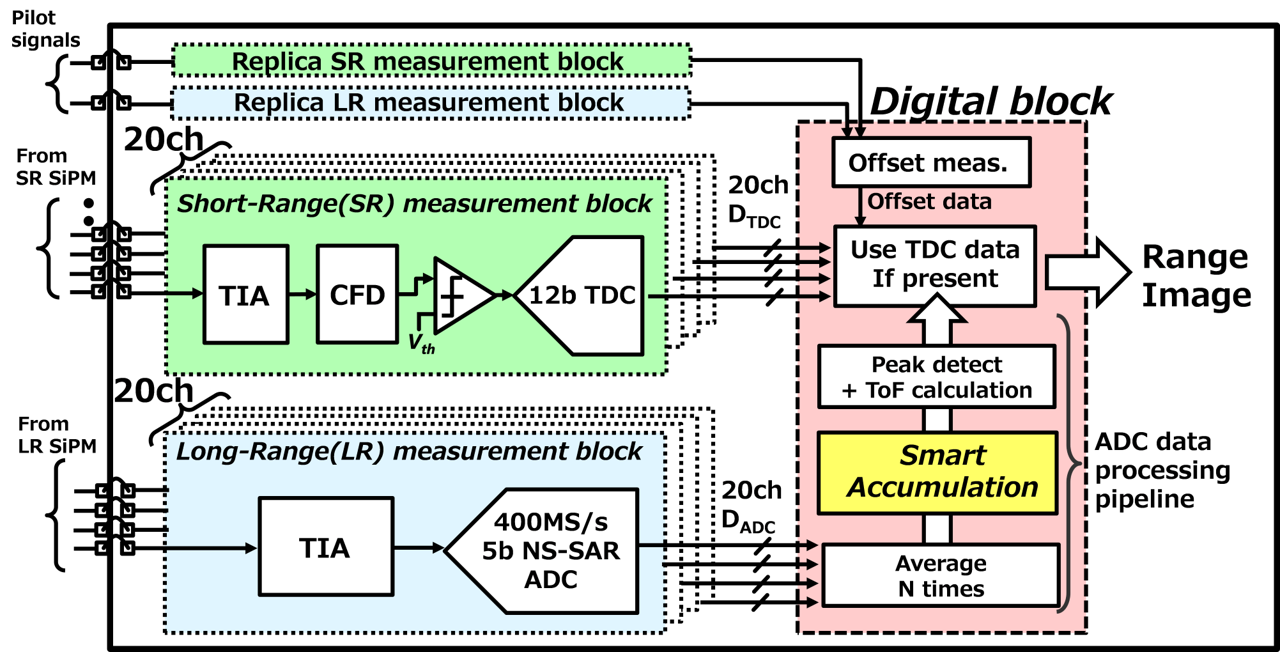
\includegraphics[width=0.5\textwidth]{figs/toshibasoc.png}
  \caption{Readout and signal processing LiDAR SoC in \cite{yoshioka201820}}
\label{rxchip}
\end{figure}

\begin{figure}[!t]
\centering
 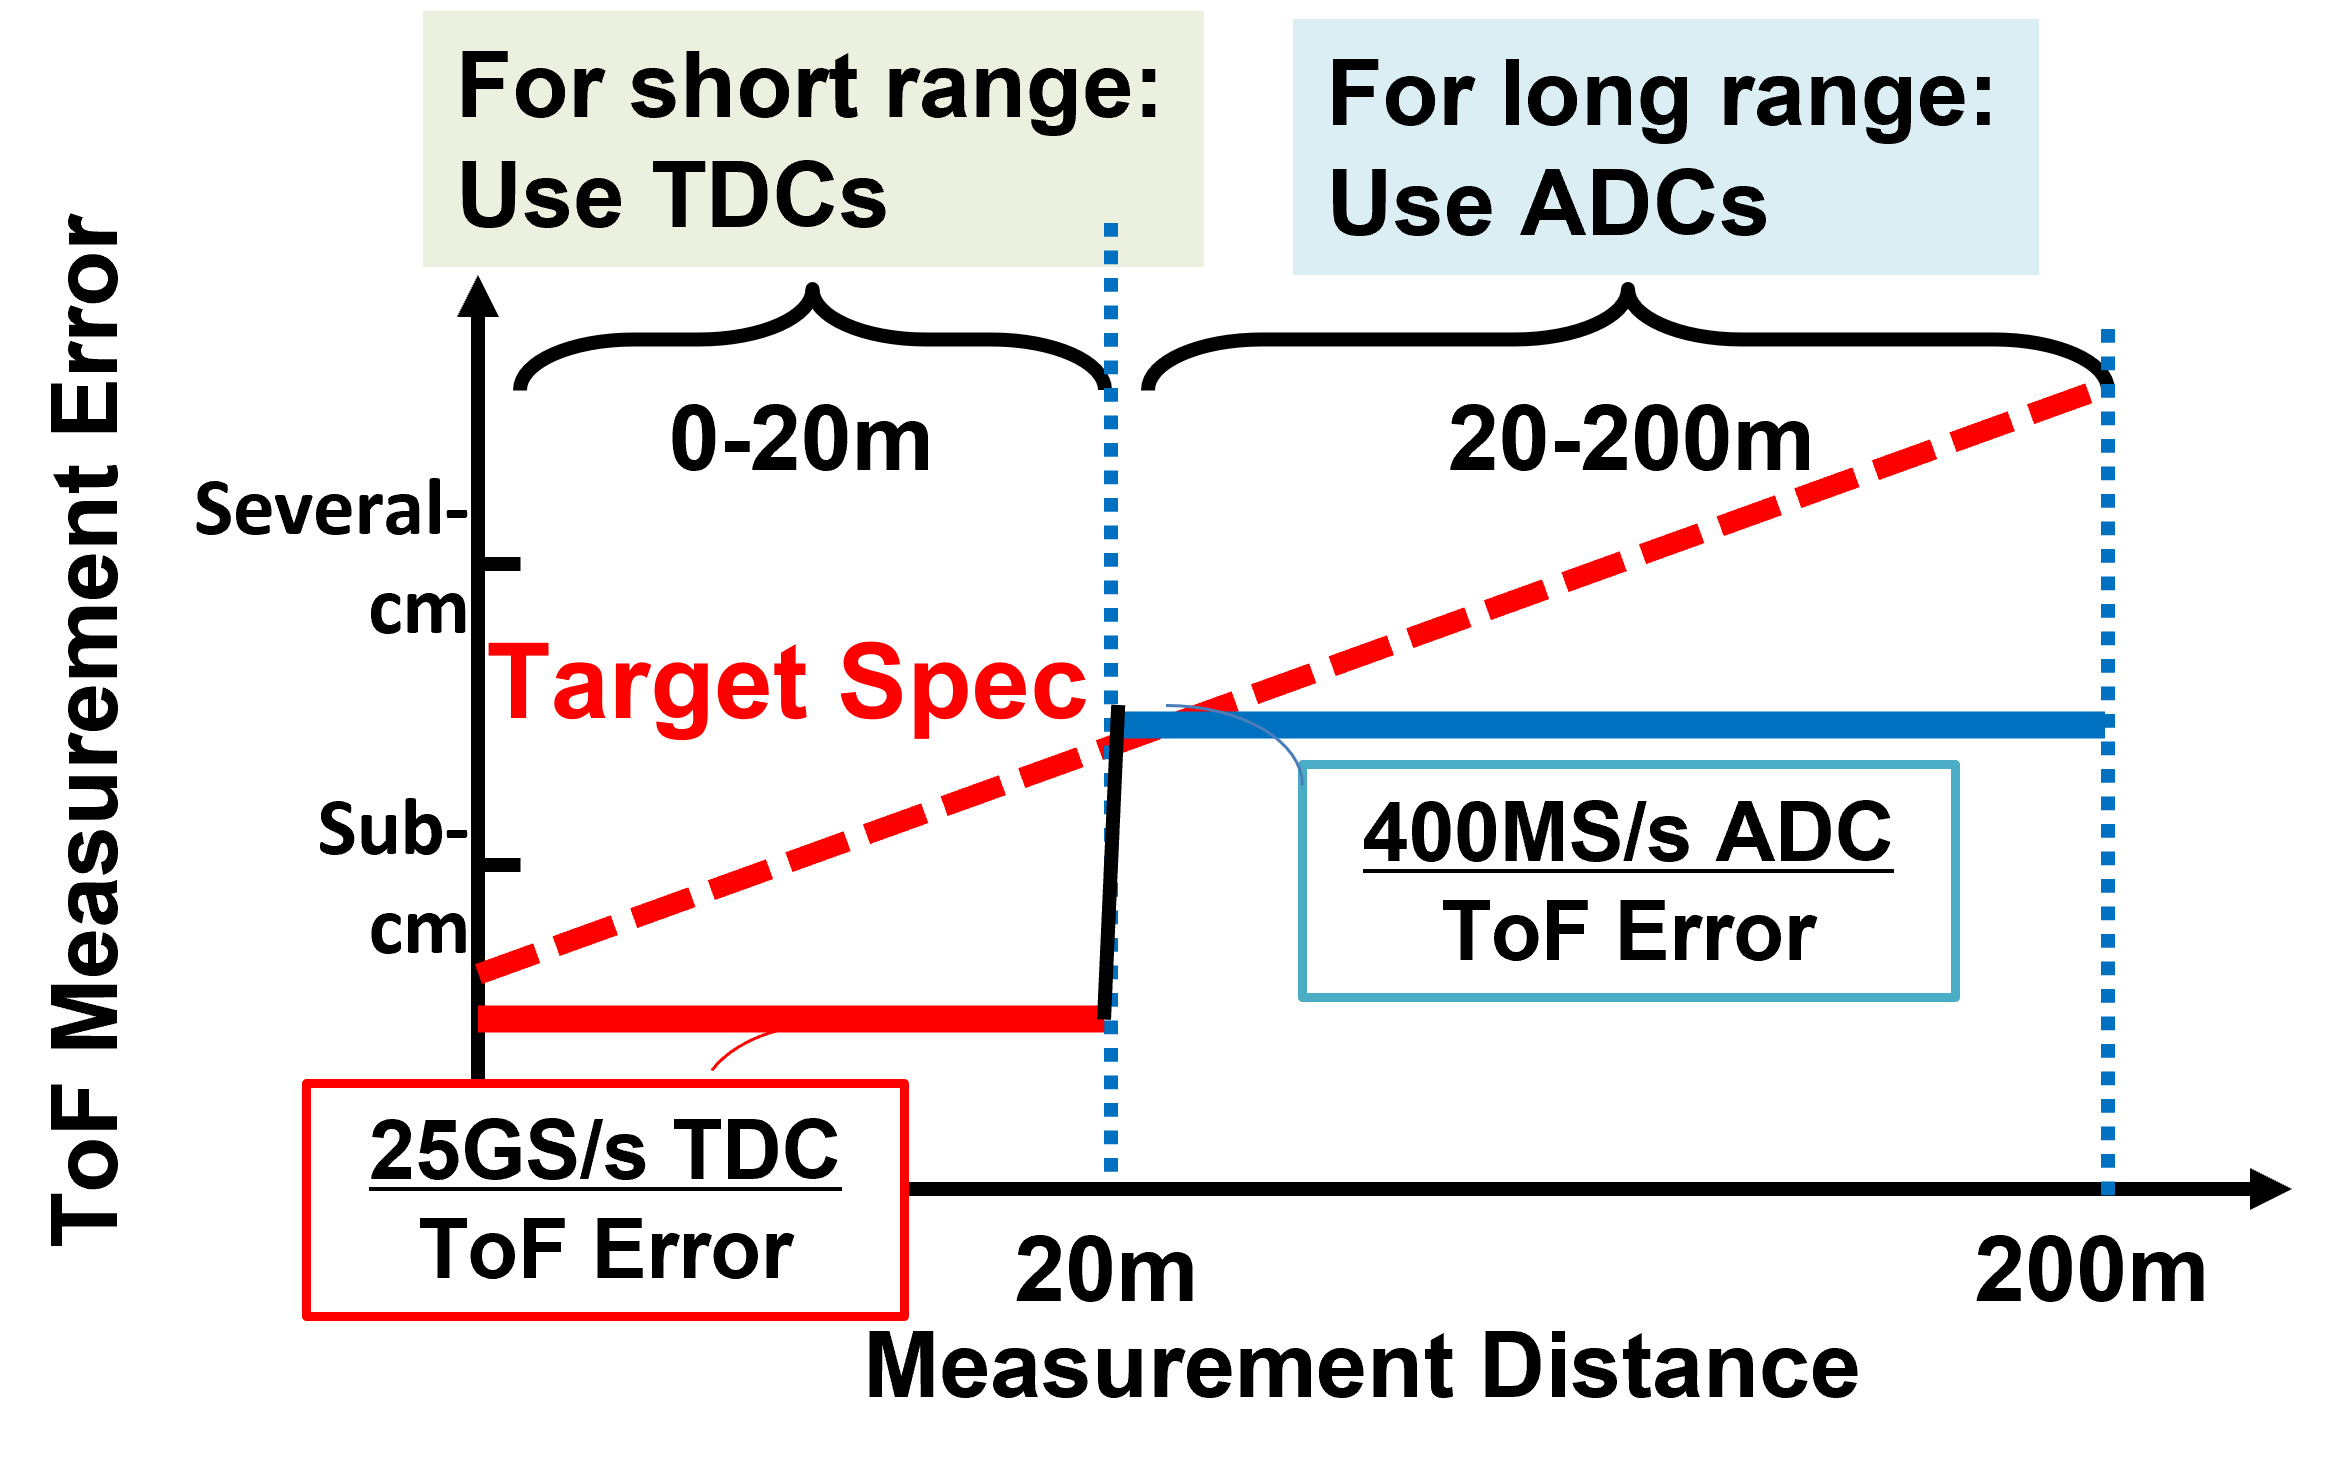
\includegraphics[width=0.5\textwidth]{figs/tdcadc.png}
  \caption{Overview of the TDC/ADC hybrid configuration. TDC with high temporal resolution is used at short range where laser is strong, and ADC is used at long range where SNR is low and accumulation is required.}
\label{tdcadc}
\end{figure}

\qquad Firstly, we will introduce the 2-chip approach.
The most distinctive feature of \cite{niclass2012100}'s architecture is that it integrates both digital and SPADs on the same chip, which is an excellent choice in terms of cost. However, it poses a challenge when further extending the performance.
For example, a special diode structure is required to get the best performance out of SPADs, which is difficult to achieve in advanced digital CMOS processes. Therefore, \cite{niclass2012100} utilizes a legacy 180nm CMOS for the SoC. By utilizing more advanced CMOS, the signal processing capability and the time resolution of TDC can be improved by Moore's Law.

Ref.\cite{yoshioka201820}'s LiDAR adopts the  2-chip approach, which achieves the best of the two worlds by adopting the most suitable process technology for the SPAD and DSP, 300nm and 28nm respectively. 
However, the number of output wires for SPADs is significant, and simply separating the chips will cause wiring issues. For this reason, \cite{yoshioka201820} uses a SiPM configuration, which connects multiple SPADs (60 in \cite{yoshioka201820}) in parallel and extracts the output as a summed current to mitigate the wiring. In addition, when utilizing a TDC, a comparator with a set threshold is used to convert the output to pulses, allowing the same processing as the conventional TDC-based systems.

In \cite{niclass2012100}, the LiDAR SNR was improved by histogramming the TDC output of multiple measurement results.
However, since the TDC is not triggered unless the SPAD's firing exceeded a certain threshold, the accumulation was not effective when the returning laser was very weak at a long distance.
Thus, by directly accumulating the raw SPAD waveform, the LiDAR can effectively utilize the information below the threshold for accumulation.

Therefore, the LiDAR SoC \cite{yoshioka201820} aims to further improve LiDAR performance by adopting a hybrid readout circuitry, which switches between ADC and TDC for far and short distances, respectively (Fig.\ref{rxchip}). 
Fig.\ref{tdcadc} illustrates the concept of the hybrid readout; a TDC is utilized for short distance measurements since high distance resolution is required and the SNR is sufficiently high. In contrast, at long distances ($>$20m) where SNR is challenging, the SiPM waveform is directly read out by an ADC, and accumulation is done in the raw waveform level. Notably, the distance resolution requirement is relaxed at longer distances so that even an ADC of 400 MS/s can achieve sufficient distance measurement performance. As a result, the TDC/ADC hybrid architecture significantly reduces the ADC speed requirement and minimizes the hardware cost. \cite{yoshioka201820} achieves 200m distance measurement for the first time due to the ADC-based waveform accumulation and custom SPAD integration.

\subsection{2D SPAD array approach}
\begin{figure}[!t]
\centering
 \includegraphics[width=0.5\textwidth]{figs/tan.png}
  \caption{2 chip system in \cite{ta20202d}.}
\label{tan}
\end{figure}

\begin{figure}[!t]
\centering
 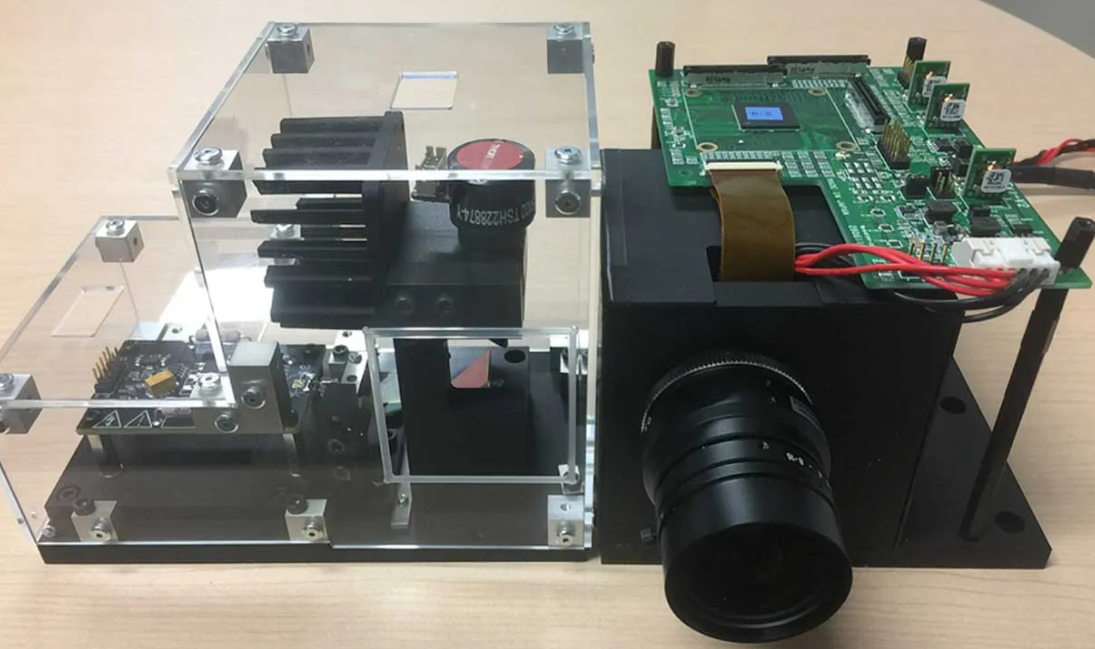
\includegraphics[width=0.4\textwidth]{figs/toshiba-proto.png}
  \caption{2D array approach allows small LiDAR integration as in \cite{ieee}}
\label{ieee}
\end{figure}

\qquad Both \cite{niclass2012100} and \cite{yoshioka201820} required a scanning mechanism to perform raster scanning (Fig.\ref{raster}) and used SPADs arranged in a 1D array.
Although raster scanning reduces the required SPADs, it involves scanning the receiving (RX) and transmitting (TX) laser beams. Since the RX scanning mechanisms are much larger than the TX due to the larger aperture ratio, this posed a significant challenge when downscaling the LiDAR size.
\cite{ta20202d} proposed an in-sensor scanning method in which the RX raster scanning is performed within the 2D SPAD array (Fig.\ref{tan}), thus eliminating the need for RX scanning machinery.
The removal of the bulky RX scanning system dramatically reduces the LiDAR sizing (Fig.\ref{ieee}).
In addition, \cite{ta20202d} uses an active quenching technique that resets the SPADs with transistors to shorten the quenching time. This enabled the reduction of SPADs per pixel,  and \cite{ta20202d}  achieved a higher resolution LiDAR system with less cost.

\subsection{3D integration approach}
\begin{figure}[!t]
\centering
 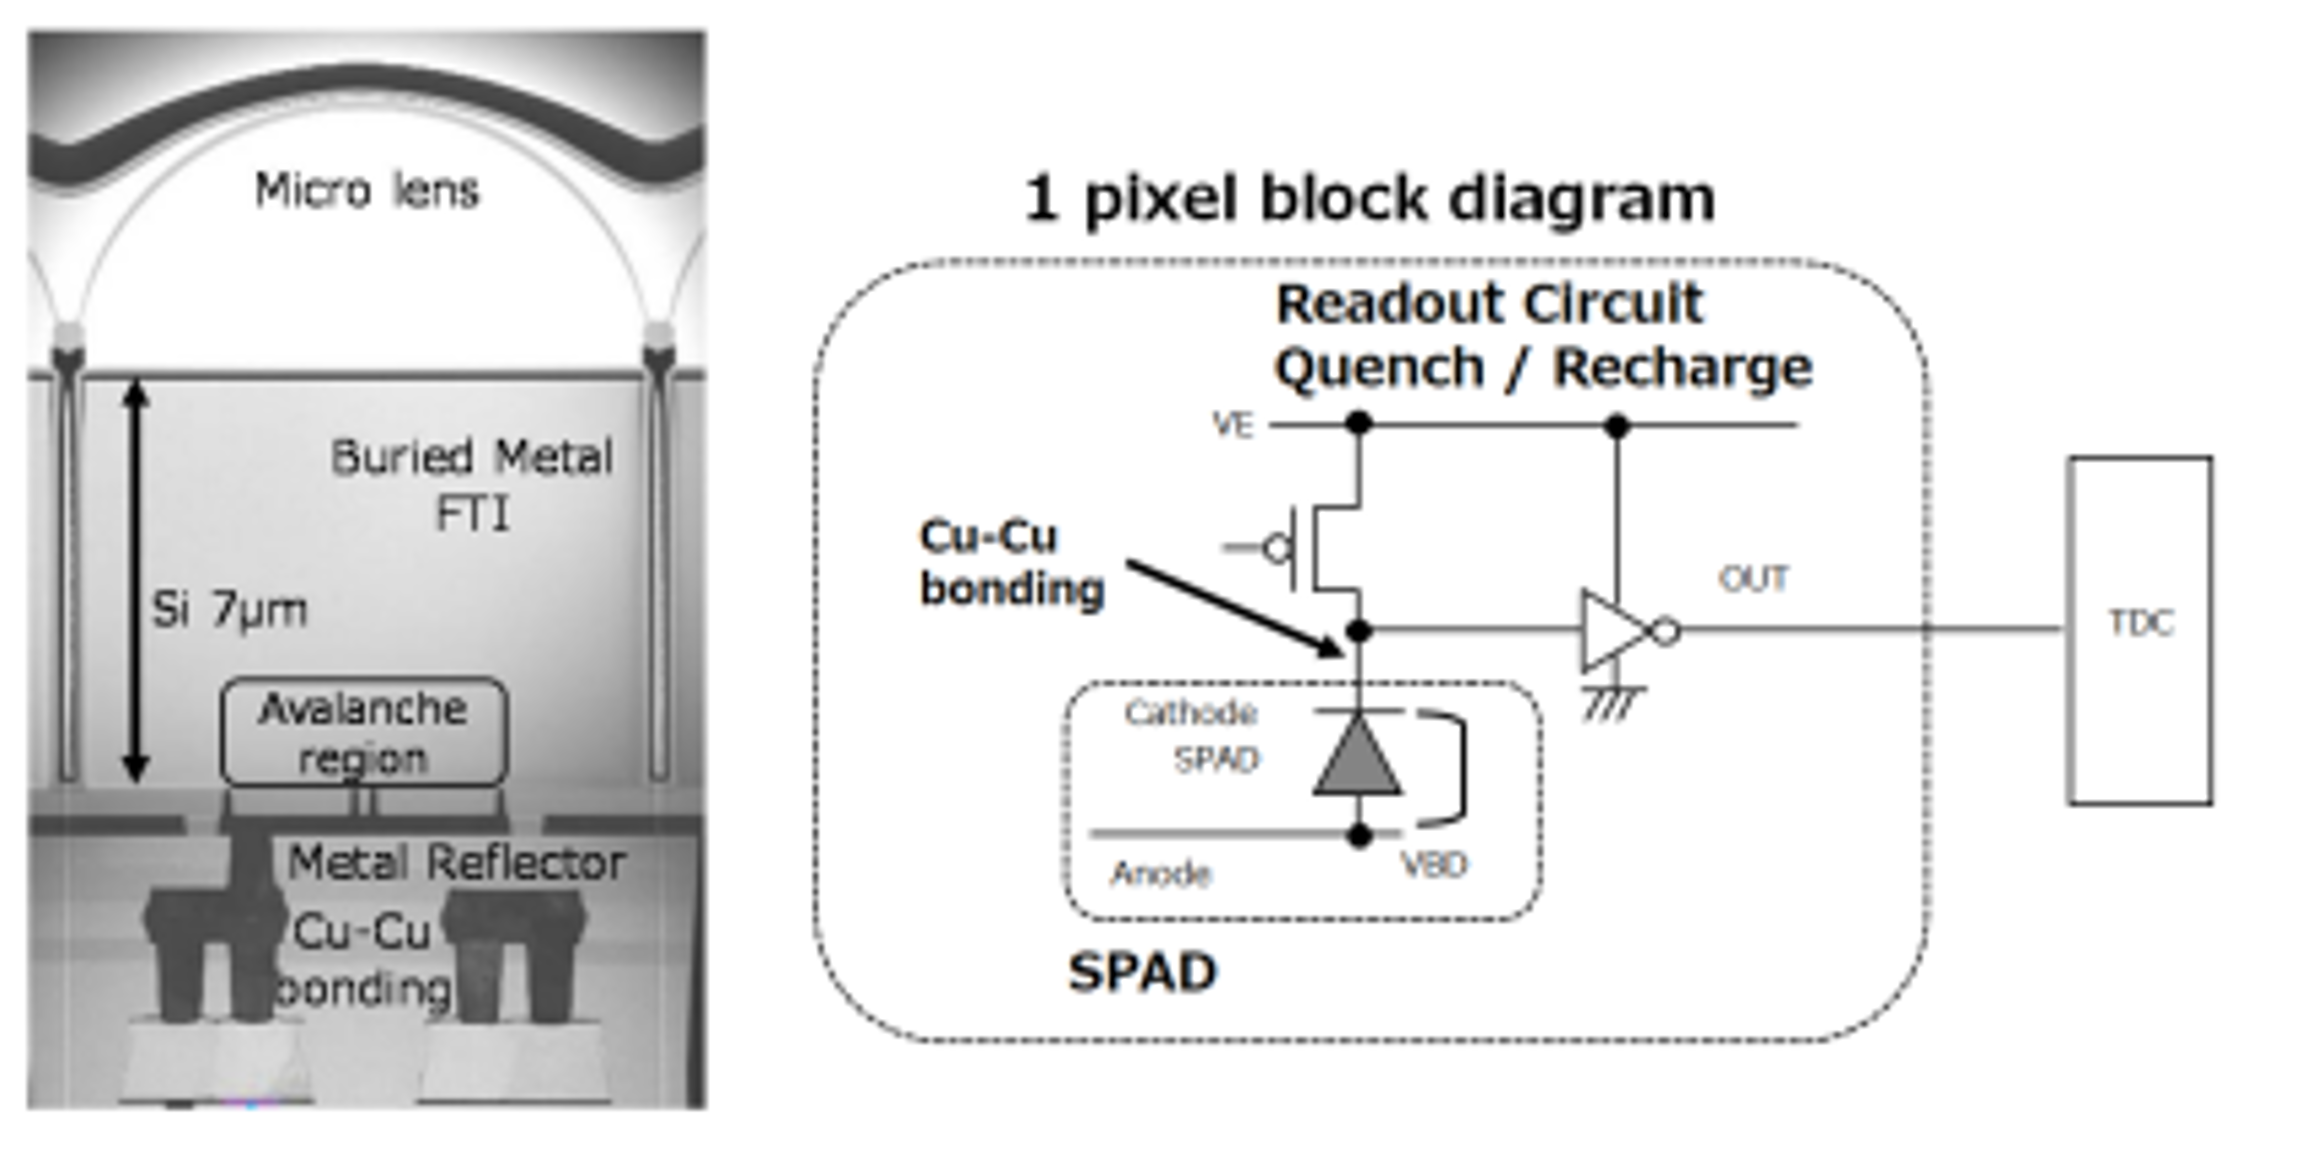
\includegraphics[width=0.5\textwidth]{figs/sonypix.png}
  \caption{3D integrated SPADs \cite{ito2020back}}
\label{sony3d}
\end{figure}

\begin{figure}[!t]
\centering
 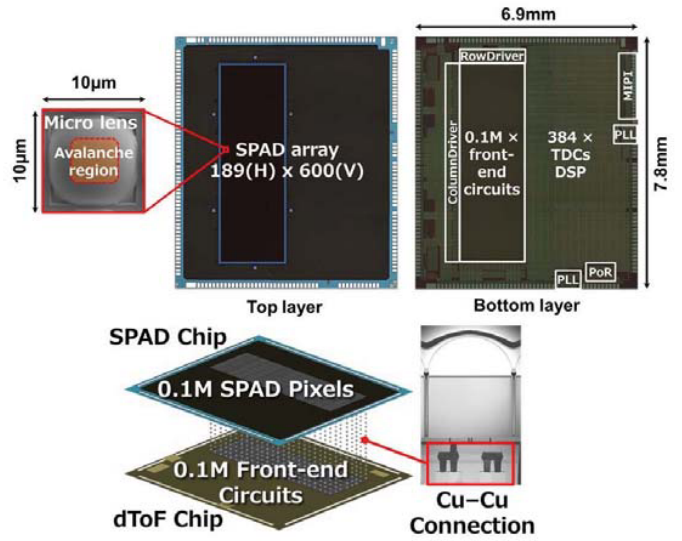
\includegraphics[width=0.5\textwidth]{figs/sony}
  \caption{3D integrated LiDAR SoC in \cite{kumagai2021189x600}}
\label{sony}
\end{figure}

\qquad Previous studies showed improved performance by fabricating the SPADs and DSP separately with suitable processes. On the other hand, as the number of pixels increases, the interchip connectivity becomes an issue and such approaches lose scalability. In addition, the SiPM connection required an ADC with low area efficiency compared to TDC. To address this issue, \cite{kumagai2021189x600, ito2020back} proposed a LiDAR SoC using the 3D integration approach as in image sensors (Fig.\ref{sony3d}, \ref{sony}). 
The 3D integration allows SPAD and DSP chips to be fabricated in a suitable process (90nm and 40nm, respectively). In addition, the large number of high-density interchip connections enabled the wiring of 100,000 SPADs.
In addition, another breakthrough is the adoption of microlens and backside illumination (BSI) technology on the SPADs. While a standard technology for increasing the sensitivity of image sensors, by applying to SPADs, the PDE dramatically improved to 22\% at 905 nm wavelength, contributing to higher LiDAR performance.

\begin{table*}[!t]
\centering
\caption{Performance comparison of first-generation and next-generation LiDARs}
 
\includegraphics[width=0.9\textwidth]{figs/performance.png}
\label{perf}
\end{table*}

Finally, we compare the performance of the LiDARs mentioned above in Table\ref{perf}. It is difficult to directly compare its performance, since they all have different scanning methods, optics, laser power, and resolutions. For example, the SNR of a MEMS mirror is lower than that of a rotating mirror, which is a disadvantage for LiDAR long-range performance (however, they accomplish much smaller LiDAR sizing). Therefore, rather than the absolute value of the LiDAR performance, it is necessary to evaluate the advancement of the circuit and system technology in this field.

\section{Conclusions and future prospects}
\qquad A tutorial and review of LiDAR for dToF ADAS were presented, where LiDARs are key distance sensors upon realizing automated driving systems. First, we discussed the breakthrough in next-generation LiDARs through comparison with the first-generation LiDAR systems. Next-generation LiDAR systems significantly improved their cost and performance by integrating the photodetector, the readout circuit, and the signal processing unit into a single SoC.
In addition, we discussed the latest developments in this field by discussing the newest research examples such as the two-chip approach, 2D SPAD array, and 3D integration LiDAR.

There are two main directions for the future development of LiDAR: commercial and research. DToF automotive LiDAR will extend its performance by evolving the SPAD and DSP performance through 3D integration and extensive signal processing. When the mass producibility of dToF LiDAR reaches a sufficient level, such LiDARs will be installed in ADAS systems of commercial vehicles.

As for research, the 1550nm LiDAR still has excellent potential. For example, dToF LiDARs have the risk of being spoofed by malicious attackers \cite{sun2020towards, cao2019adversarial}, and there are high hopes for FMCW LiDARs that can prevent this from happening \cite{aptivpatent}. In addition, 1550nm LiDARs with silicon photonics can realize solid-state laser scanning to scale the cost further, and the research development attracts significant attention\cite{poulton2017coherent}.

%自動運転システムの距離センサとして中核的な役割を果たすdToF ADAS用LiDARについて議論を行った。黎明期の第一世代LiDAR、そしてシステムをチップ上に集積することでコストと性能を大きく改善した次世代LiDARについてreviewを行った。特に次世代LiDARの主な進歩要因を受光素子、読み出し回路、及び信号処理部の集積化と捉えそれぞれの回路システムについてディスカッションを行った。加えて2チップアプローチ、2D SPADアレー、そして3DインテグレーションLiDARといった最新の研究例のディスカッションを行うことで本分野の最新の発展について議論した。

%今後のLiDARの発展には商用と研究で大きく2つの方向性がある。商用には3Dインテグレーションやより微細プロセスを用いることで更にSPAD性能やDSP性能を向上させることでdToF車載LiDARの性能発展が見込まれる。そして十分に信頼性や量産性が確保されたのであれば市販車のADASシステムに搭載される日も遠くないと筆者は考えている。

%また研究としては1550nm LiDARに大きな可能性が残されている。特にdToF LiDARは悪意を持った攻撃者にハッキングされる危険性があり\cite{sun2020towards, cao2019adversarial}、これを防ぐことのできるFMCW LiDARに期待が集まっている\cite{aptivpatent}。またシリコンフォトニクスを用いたLiDARは送信側のレーザ走査をもsolid-state化することが期待され研究の発展動向に注目している\cite{poulton2017coherent,chung202119}。

\section*{Acknowledgements}
This work was supported in part by the JST CREST program under Grant JPMJCR21D2, and in part by the Japan Society for the Promotion of Science (JSPS) KAKENHI, under Grant 21K20413.

\bibliographystyle{IEEEbib}
\bibliography{main}


\begin{IEEEbiography}
[{
\includegraphics[width=1in,height=1.25in,clip,keepaspectratio]{bio/1.jpg}}]{Kentaro Yoshioka}
received his BS, MS, Ph.D degrees from Keio University, Japan. Currently, he is an Assistant Professor at Keio University. He worked with Toshiba during 2014-2021, developing circuitry for WiFi and LiDAR SoCs. During 2017-2018, he had been a visiting scholar at Stanford University, exploring efficient machine learning hardware and algorithms. 

Currently, Dr. Yoshioka serves as a technical program member of Symp. VLSI circuits conference. He was the recipient of ASP-DAC 2013 Special Feature Award, the A-SSCC 2012 Best Design Award, and 1st place winner of Kaggle 2020 Prostate Cancer Grade Assessment (PANDA) Challenge.
\end{IEEEbiography}

\end{document}
